\documentclass[lang=cn,11pt,a4paper,cite=authornum]{paper}

\title{数据库系统原理 实验一、实验二、实验三 \\ 实验报告}
\author{毛子恒 \\ 2019211397}
\institute{北京邮电大学\ 计算机学院}

\date{\zhtoday}

% 本文档命令
\nocite{*}

\begin{document}

\maketitle

\part{实验一}

\section{概述}

\subsection{实验目的}

\begin{enumerate}
    \item 通过对GaussDB(for openGauss)数据库创建与访问:
          \begin{enumerate}
              \item 了解华为云分布式数据库GaussDB(for openGauss)的软件环境和创建方法;
              \item 掌握并熟悉GaussDB(for openGauss)数据库软件的使用方法;
              \item 掌握并熟悉GaussDB(for openGauss)数据库软件的构成和相关工具;
              \item 通过GaussDB(for openGauss)数据库软件的使用,深入理解数据库系统的基本概念。
          \end{enumerate}
    \item 通过创建GaussDB(for openGauss)数据库及进行相应的维护,了解并掌握GaussDB(for openGauss)数据库的创建与维护的不同方法和途径,进而通过这一具体的数据库理解实际数据库所包含的各要素。
\end{enumerate}

\subsection{实验平台及环境}

\begin{itemize}
    \item 华为云GaussDB(for openGauss) 1.4.1
    \item 数据库兼容:PostgreSQL
\end{itemize}

\subsection{实验内容}

\begin{enumerate}
    \item GaussDB(for openGauss)数据库软件的使用:
          \begin{enumerate}
              \item 登录并运行GaussDB(for openGauss)数据库;
              \item 了解华为云数据库GaussDB(for openGauss)的机制;
              \item 熟悉GaussDB(for openGauss)数据库的各项功能。
          \end{enumerate}
    \item 数据库创建与维护:
          \begin{enumerate}
              \item 创建“疫情数据”数据库;
              \item 对数据库属性和参数进行相应的修改和维护;
              \item 练习数据库的删除等维护操作。
          \end{enumerate}
\end{enumerate}

\subsection{实验步骤}

\begin{enumerate}
    \item 熟悉GaussDB(for openGauss)数据库的创建过程。
    \item 创建一个名为“疫情数据”的数据库;
    \item 删除“疫情数据”数据库。
\end{enumerate}

\section{实验结果及分析}

\paragraph{数据库的登录}

\begin{enumerate}
    \item 登录华为云控制台,进入数据库管理服务器DAS;
    \item 进入开发工具;
    \item 新增数据库实例登录,数据库引擎设置为GaussDB(for openGauss),设置用户名和密码;
    \item 登录刚才创建的数据库实例。
\end{enumerate}

\paragraph{数据库的创建}

新建数据库,命名为"Epidemic\_data2019211397",如\figref{fig:create_db}。
\begin{figure}[!htb]
    \centering
    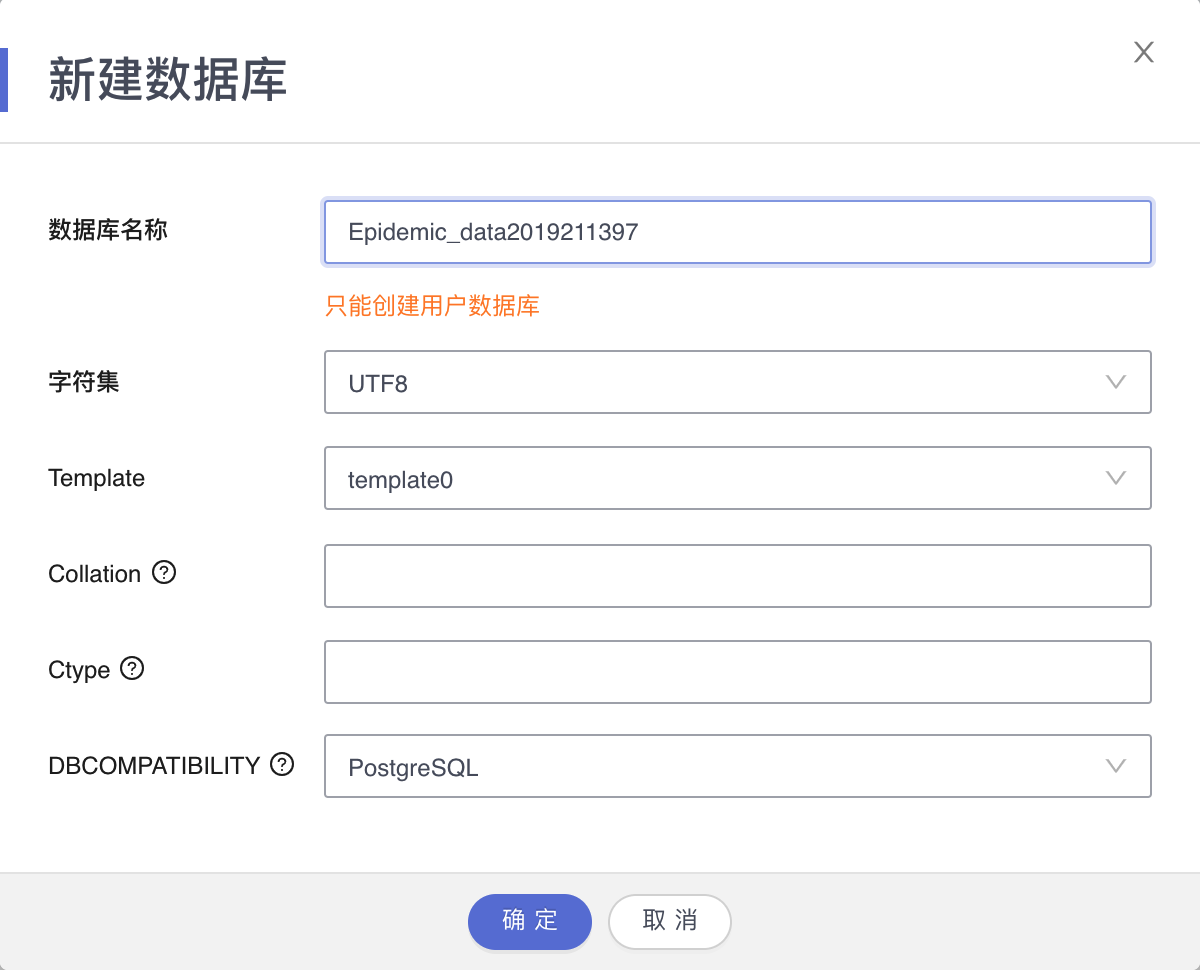
\includegraphics[width=0.5\textwidth]{./images/create_db.png}
    \caption{创建数据库\label{fig:create_db}}
\end{figure}

对应SQL语句为:

\begin{code}
\begin{minted}{sql}
CREATE DATABASE Epidemic_data2019211397;
\end{minted}
\end{code}

\paragraph{数据库的删除}

点击“删除库”,如\figref{fig:delete_db}。
\begin{figure}[!htb]
    \centering
    
\includegraphics[width=\textwidth]{./images/delete_db.png}
    \caption{删除数据库\label{fig:delete_db}}
\end{figure}

对应SQL语句为:

\begin{code}
\begin{minted}{sql}
DROP DATABASE Epidemic_data2019211397;
\end{minted}
\end{code}

\section{实验总结}

本次实验中我基本熟悉了华为云数据库的使用,在IAM账号下进行了数据库的创建和删除操作,期间依照实验步骤进行操作,没有问题产生。

\part{实验二}

\section{概述}

\subsection{实验目的}

\begin{enumerate}
    \item 通过进行数据库表的建立操作,熟悉并掌握GaussDB(for openGauss)数据库表的建立方法,理解关系型数据库表的结构,巩固PostgreSQL中关于数据库表的建立语句;
    \item 通过进行数据库表数据的增加、删除和插入等维护操作,熟悉并掌握GaussDB(for openGauss)数据库数据的操作方法,巩固PostgreSQL中关于数据维护的语句。
\end{enumerate}

\subsection{实验平台及环境}

\begin{itemize}
    \item 华为云GaussDB(for openGauss) 1.4.1
    \item 数据库兼容:PostgreSQL
\end{itemize}

\subsection{实验内容}

建立相应的表并熟悉基本操作,例如建表、对表进行增、删、改、查。

\subsection{实验步骤}

\begin{enumerate}
    \item 熟悉课程实验背景知识;
    \item 使用GaussDB(for openGauss)数据库软件创建相应的表;
    \item 将提供的数据导入各表,掌握GaussDB(for openGauss)数据库数据导入的方法;注意:
    \begin{enumerate}
        \item 表中空列的处理;
        \item 表结构与数据类型的匹配。
    \end{enumerate}	
    \item 修改 “病例基本信息”表数据,增加名为“备注”的列,数据类型为\mintinline{sql}{varchar()}型。
    \item 修改 “病例基本信息”表数据,将 “备注”列的数据类型改为\mintinline{sql}{int}。
    \item 修改 “病例基本信息”表数据,删除“备注”列。
    \item 删除“病例基本信息”数据表。
\end{enumerate}

\section{实验结果及分析}

\paragraph{数据表的创建}

观察数据表的结构,执行如下SQL语句来创建表:

\begin{code}
\begin{minted}{sql}
CREATE TABLE 病例行程信息表 (
    行程号 INTEGER NULL,
    病例号 INTEGER NULL,
    日期信息 VARCHAR(100) NULL,
    行程信息 VARCHAR(250) NULL
);
CREATE TABLE 美国各州县确诊与死亡数统计表 (
    日期 DATE NULL,
    国家 VARCHAR(50) NULL,
    州 VARCHAR(50) NULL,
    县 VARCHAR(50) NULL,
    累计确诊 INTEGER NULL,
    累计死亡 INTEGER NULL
);
CREATE TABLE 全国各省累计数据统计表 (
    日期 DATE NULL,
    省 VARCHAR(50) NULL,
    累计确诊 INTEGER NULL,
    累计治愈 INTEGER NULL,
    累计死亡 INTEGER NULL
);
CREATE TABLE 病例基本信息表 (
    病例号 INTEGER NULL,
    省 VARCHAR(50) NULL,
    市 VARCHAR(50) NULL,
    区 VARCHAR(50) NULL,
    日期 DATE NULL,
    性别 VARCHAR(50) NULL,
    年龄 INTEGER NULL,
    患者信息 VARCHAR(100) NULL,
    其他信息 VARCHAR(200) NULL,
    信息来源 VARCHAR(50) NULL
);
CREATE TABLE 参考信息表 (
    组合码 VARCHAR(100) NULL,
    国家地区 VARCHAR(50) NULL,
    省州 VARCHAR(50) NULL,
    市县 VARCHAR(50) NULL,
    纬度 DOUBLE PRECISION NULL,
    经度 DOUBLE PRECISION NULL,
    人口数 INTEGER NULL
);
CREATE TABLE 各国疫情数据统计表 (
    日期 DATE NULL,
    国家地区 VARCHAR(50) NULL,
    省州 VARCHAR(50) NULL,
    累计确诊 INTEGER NULL,
    累计治愈 INTEGER NULL,
    累计死亡 INTEGER NULL
);
CREATE TABLE 全国城市风险等级表 (
    省 VARCHAR(50) NULL,
    市 VARCHAR(50) NULL,
    区 VARCHAR(50) NULL,
    地址详情 VARCHAR(100) NULL,
    风险等级 VARCHAR(50) NULL
);
CREATE TABLE 全国各省参考信息表 (
    中文名称 VARCHAR(50) NULL,
    英文名称 VARCHAR(50) NULL,
    组合码 VARCHAR(50) NULL,
    纬度 DOUBLE PRECISION NULL,
    经度 DOUBLE PRECISION NULL,
    人口数 INTEGER NULL
);
\end{minted}
\end{code}

\paragraph{导入各表}

点击数据管理服务中的“导入”菜单,点击“新建任务”,选择CSV附件,上传文件,选择对应的数据库和表,执行导入任务,如\figref{fig:import}。

\begin{figure}[!htb]
    \centering
    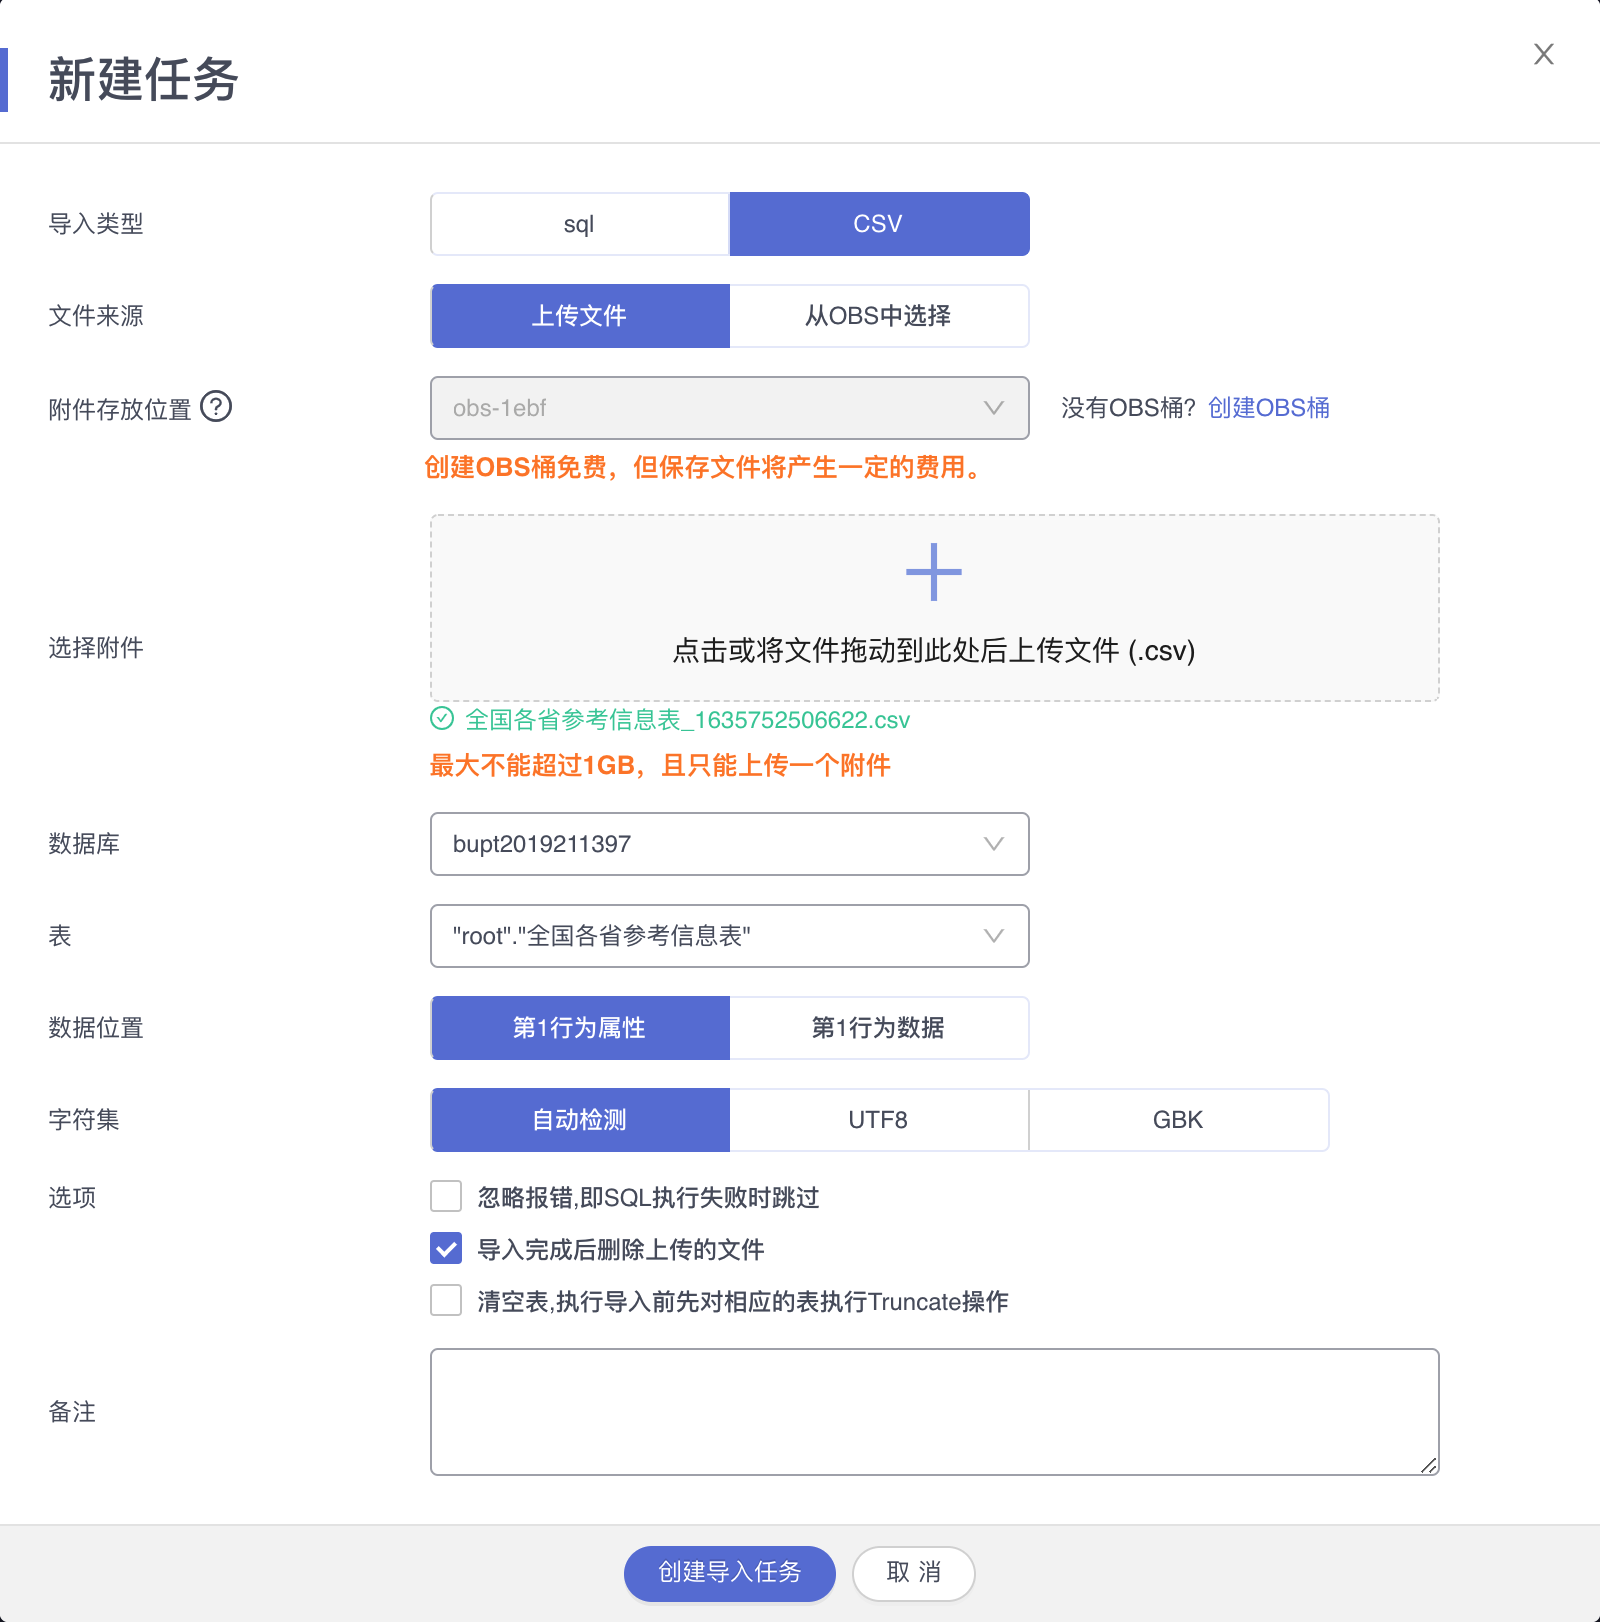
\includegraphics[width=0.6\textwidth]{./images/import.png}
    \caption{导入表\label{fig:import}}
\end{figure}

对于存在空列(集包括列头的整列都为空)的表,利用Excel将空列删除即可。

\paragraph{修改“病例基本信息”表数据}

增加名为“备注”的列,数据类型为\mintinline{sql}{varchar()}。

\begin{code}
\begin{minted}{sql}
ALTER TABLE 病例基本信息表 ADD 备注 varchar(100);
\end{minted}
\end{code}

将“备注”列的数据类型改为\mintinline{sql}{int}。

\begin{code}
\begin{minted}{sql}
ALTER TABLE 病例基本信息表 ALTER COLUMN 备注 TYPE INTEGER;
\end{minted}
\end{code}

删除“备注”列。

\begin{code}
\begin{minted}{sql}
ALTER TABLE 病例基本信息表 DROP COLUMN 备注;
\end{minted}
\end{code}

\paragraph{删除“病例基本信息”数据表} SQL语句如下:

\begin{code}
\begin{minted}{sql}
DROP TABLE 病例基本信息表;
\end{minted}
\end{code}

\section{实验总结}

在导入数据的过程中,出现导入错误的情况,经查看错误日志,大部分情况都是\mintinline{sql}{varchar}的长度限制太小所致,增大长度限制之后即可正常导入。

在导入过程中注意细分列的类型,比如病例形成信息表的形成号和病历号设为\mintinline{text}{int}类型,日期列都设为\mintinline{text}{date}类型,这样有助于后续的查询操作。

实验使我对基本的SQL建表和修改表的操作更加熟悉,实验过程中没有遇到其它问题。

\part{实验三}

\section{概述}

\subsection{实验目的}

通过对实验二建立的数据库关系表的各种查询的操作,加深对SQL语言和PostgreSQL查询语言的了解,掌握相关查询语句的语法及使用方法。

\subsection{实验平台及环境}

\begin{itemize}
    \item 华为云GaussDB(for openGauss) 1.4.1
    \item 数据库兼容:PostgreSQL
\end{itemize}

\subsection{实验内容}

\subsubsection{单表查询}

\begin{enumerate}
    \item 查询国内确诊病例基本信息的所有信息来源;
    \item 给出河南省、西藏自治区、台湾省的英文名称和人口数;
    \item 查询2021年1月20日各省现有确诊病例数据,按现有确诊病例数降序排列输出。计算方法:现有确诊数=累计确诊-累计死亡-累计治愈;
    \item 计算截至2021年1月20日全国累计确诊病例数;
    \item 查询1005号病例确诊后,其所在市新增的所有确诊病例;
    \item 在“病例基本信息表”中查询石家庄市在2021年1月11日当天以及之前的所有60岁以上的患者信息;
    \item 统计截止到2020年12月30日美国累计确诊病例数最多的10个州;
    \item 统计截止到2020年12月30日美国新冠疫情死亡率高于2\%的州。
\end{enumerate}

\subsubsection{多表查询}

\begin{enumerate}
    \item 借助病例行程信息粗略查询曾去过“源升品质生活坊”的所有患者的基本信息;
    \item 根据病例行程信息表和病例基本信息表,查询行程信息中存在“家庭聚餐”的病例被确诊的日期;
    \item 对比中美两国累计确诊病例数,输出格式为(日期,中国累计确诊,美国累计确诊);
    \item 计算截止到2021年1月20日,美国有些县的累计确诊是同一个州的其他县的2倍或以上,列出这些县,以及他们所在的州和他们的累计确诊;
    \item 计算世界上人口数排名前10位的国家地区;
    \item 列出美国人口超千万的大州中,截至2021年1月20日新冠肺炎疫情死亡率超过2\%的州;
    \item 截至2021年1月20日,河北省哪些区出现了新冠确诊病例但不属于中高风险地区;
    \item 在病例行程信息表的基础上根据病例基本信息表,查询河北省病例的信息:包括行程ID,病例ID,患者信息,日期信息,行程信息。
\end{enumerate}

\subsubsection{嵌套查询}

\begin{enumerate}
    \item 查询披露的确诊患者信息中年龄最大的患者,输出其基本信息。(未注明年龄的患者不进行比较);
    \item 查询2020年12月份新增确诊患者最多的城市;
    \item 结合“全国各省参考信息表”和“病例基本信息表”给出没有新增确诊病例或未披露病例信息的省份;
    \item 2021年1月20日全国中高风险地区所在省中,哪些省在1月20日没有新增确诊信息披露;
    \item 根据病例基本信息表查询一月份国内新增患者病例最多的城市;
    \item 查询除中美两国以外的其余国家中,进入2021年以来单日新增确诊病例始终不低于一万例的国家。
\end{enumerate}

\section{实验结果及分析}

\paragraph{国内确诊病例基本信息的所有信息来源} SQL语句如下:

\begin{code}
\begin{minted}{sql}
SELECT DISTINCT 信息来源
FROM 病例基本信息表;
\end{minted}
\end{code}

语句从病例基本信息表中选出不重复的信息来源。查询结果如\figref{fig:query1}。

\begin{figure}[!htb]
    \centering
    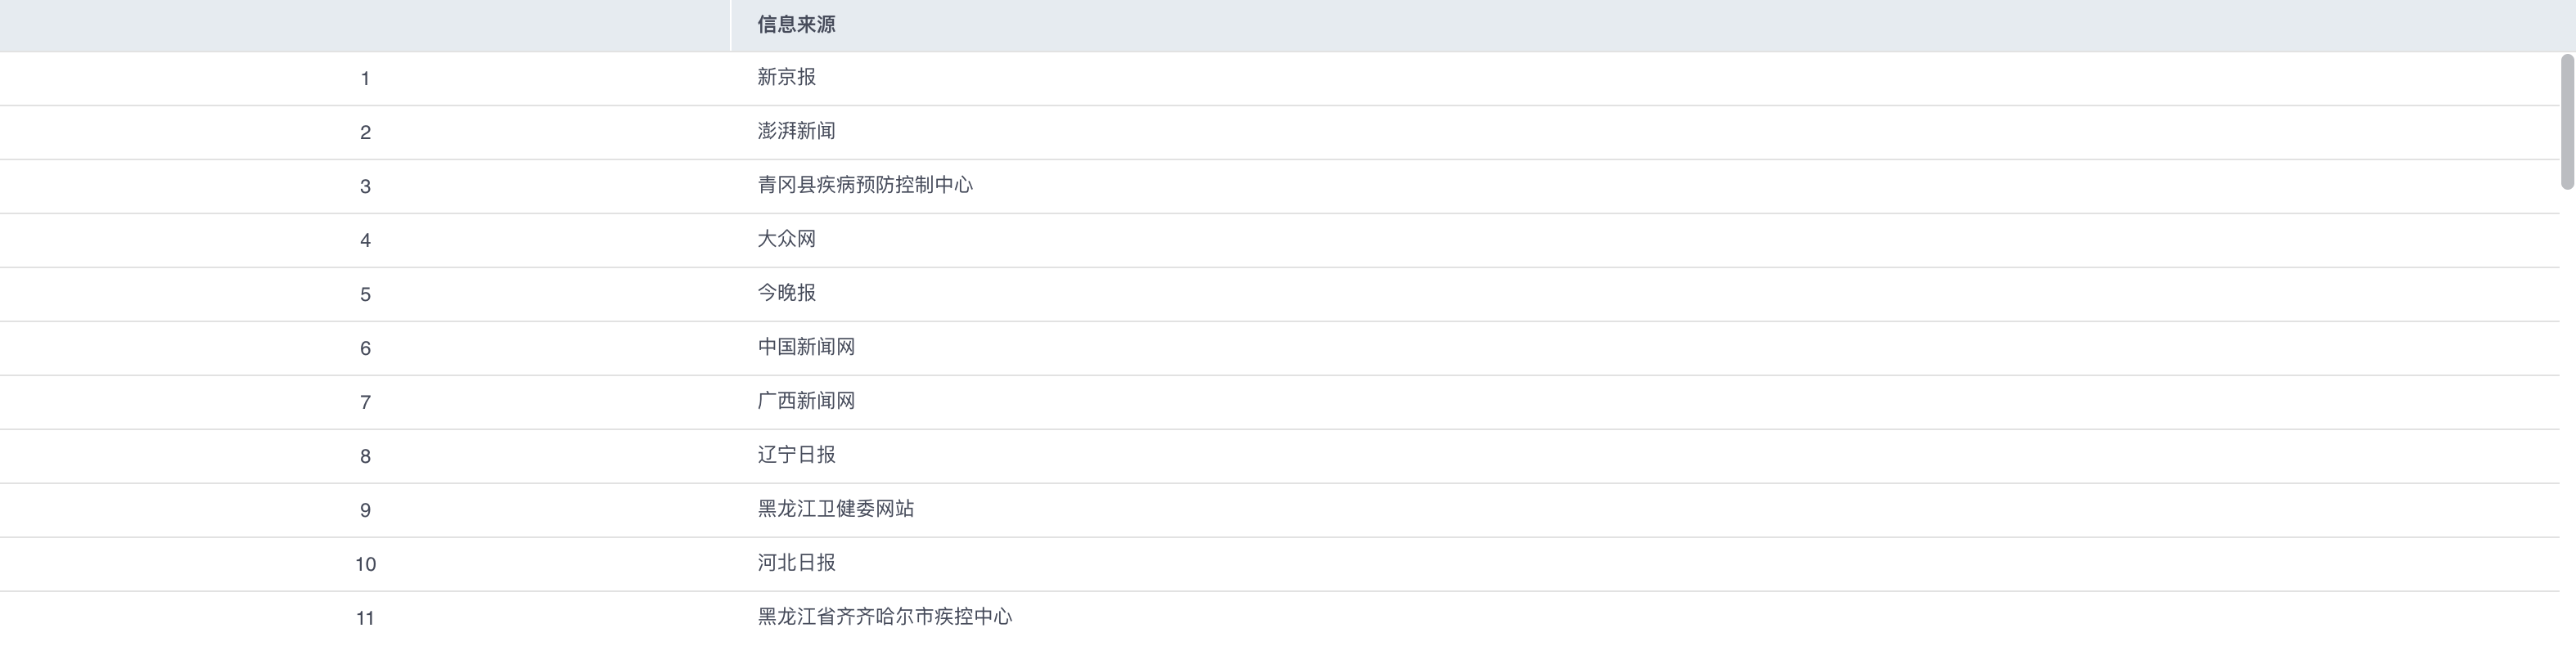
\includegraphics[width=\textwidth]{./images/lab1_query1.png}
    \caption{查询结果1\label{fig:query1}}
\end{figure}

\paragraph{河南省、西藏自治区、台湾省的英文名称和人口数} SQL语句如下:

\begin{code}
\begin{minted}{sql}
SELECT 英文名称, 人口数
FROM 全国各省参考信息表
WHERE 中文名称 IN ('河南省', '西藏自治区', '台湾省');
\end{minted}
\end{code}

语句从各省参考信息表中选出三个省的元组,再选出英文名称和人口数。查询结果如\figref{fig:query2}。

\begin{figure}[!htb]
    \centering
    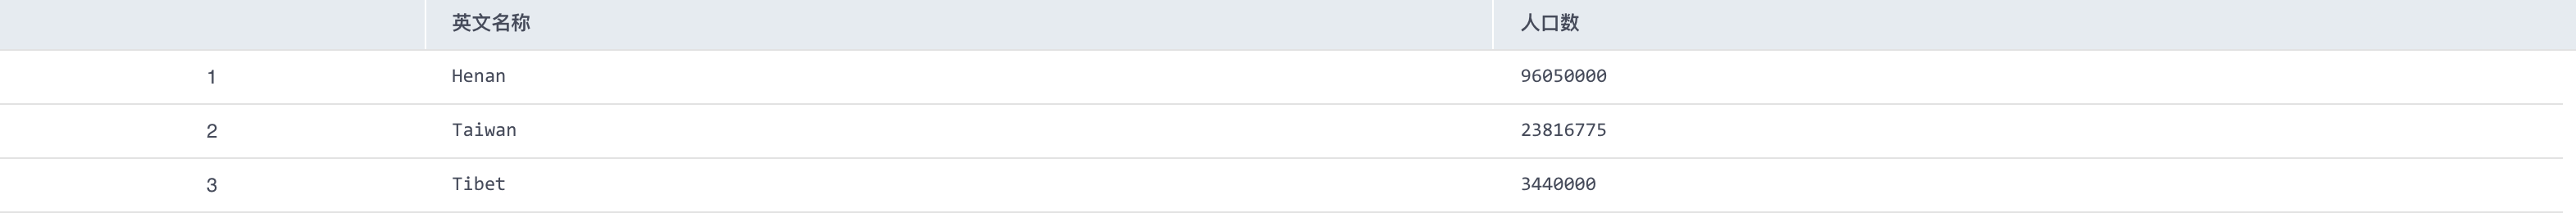
\includegraphics[width=\textwidth]{./images/lab1_query2.png}
    \caption{查询结果2\label{fig:query2}}
\end{figure}

\paragraph{2021年1月20日各省现有确诊病例数据,按现有确诊病例数降序排列输出} SQL语句如下:

\begin{code}
\begin{minted}{sql}
SELECT 省, 累计确诊-累计死亡-累计治愈 AS 现有确诊数
FROM 全国各省累计数据统计表
WHERE 日期 = '2021-01-20'
ORDER BY 现有确诊数 DESC;
\end{minted}
\end{code}

语句查询该日各省的数据,并按现有确诊数降序输出。查询结果如\figref{fig:query3}。

\begin{figure}[!htb]
    \centering
    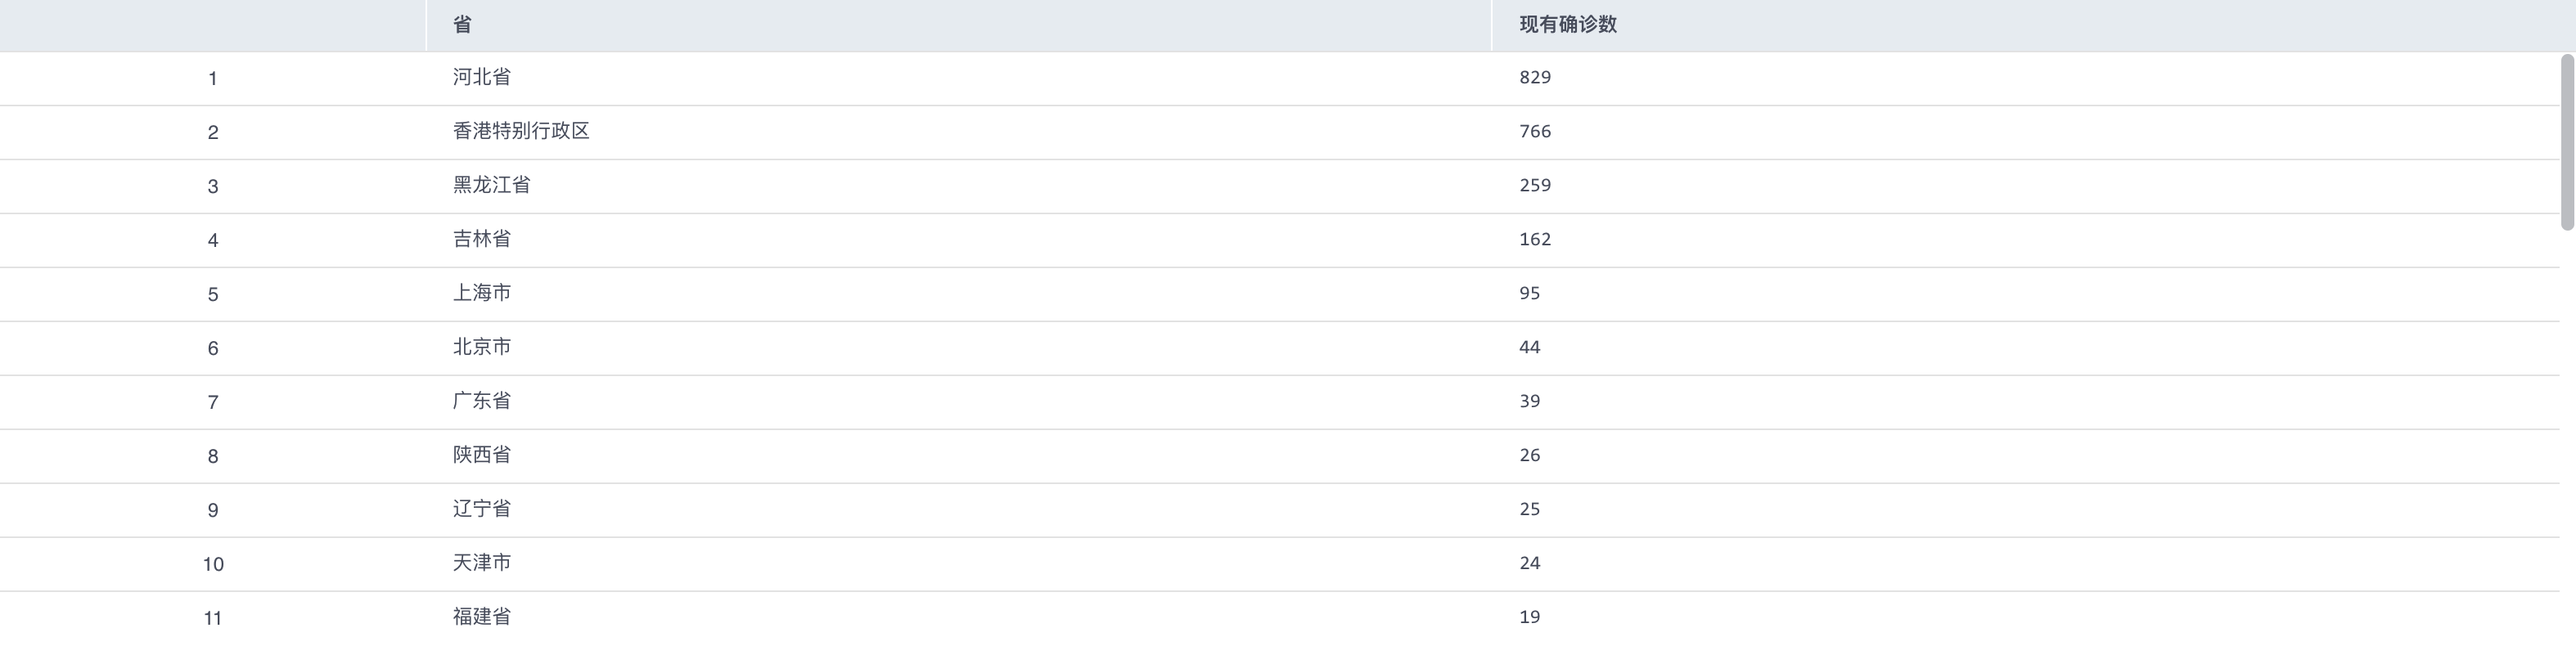
\includegraphics[width=\textwidth]{./images/lab1_query3.png}
    \caption{查询结果3\label{fig:query3}}
\end{figure}

\paragraph{截至2021年1月20日全国累计确诊病例数} SQL语句如下:

\begin{code}
\begin{minted}{sql}
SELECT SUM(累计确诊) AS 全国累计确诊病例数
FROM 全国各省累计数据统计表
WHERE 日期 = '2021-01-20';
\end{minted}
\end{code}

语句从累计数据统计表中查询当日各省的累计确诊数之和。查询结果如\figref{fig:query4}。

\begin{figure}[!htb]
    \centering
    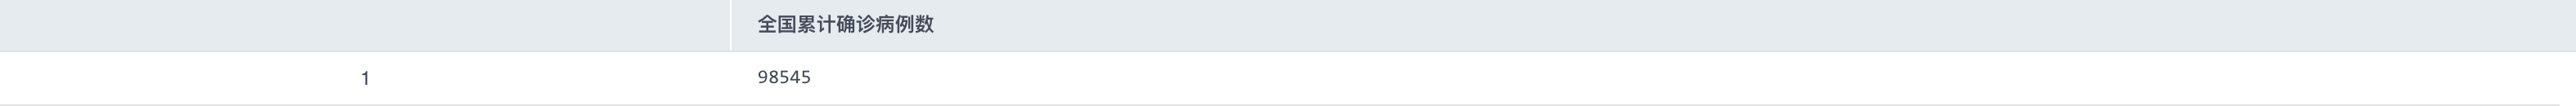
\includegraphics[width=\textwidth]{./images/lab1_query4.png}
    \caption{查询结果4\label{fig:query4}}
\end{figure}

\paragraph{1005号病例确诊后,其所在市新增的所有确诊病例} SQL语句如下:

\begin{code}
\begin{minted}{sql}
SELECT *
FROM 病例基本信息表 AS T1
WHERE EXISTS (
    SELECT 日期, 市
    FROM 病例基本信息表 AS T2
    WHERE T2.病例号 = 1005 AND T1.日期 >= T2.日期 AND T1.市 = T2.市
);
\end{minted}
\end{code}

或

\begin{code}
\begin{minted}{sql}
WITH 病例1005 AS (
    SELECT 日期, 市
    FROM 病例基本信息表
    WHERE 病例号 = 1005
)
SELECT 病例基本信息表.*
FROM 病例基本信息表, 病例1005
WHERE 病例基本信息表.日期 >= 病例1005.日期 AND 病例基本信息表.市 = 病例1005.市;
\end{minted}
\end{code}

语句利用相关子查询,从\mintinline{sql}{WHERE}子句中筛选出病例1005的关系和外层的关系比较;或者可以采用\mintinline{sql}{WITH}子句创建一个临时关系,用来表示病例1005,之后再从病例基本信息表中选取元组和这个关系进行比较。查询结果如\figref{fig:query5}。

\begin{figure}[!htb]
    \centering
    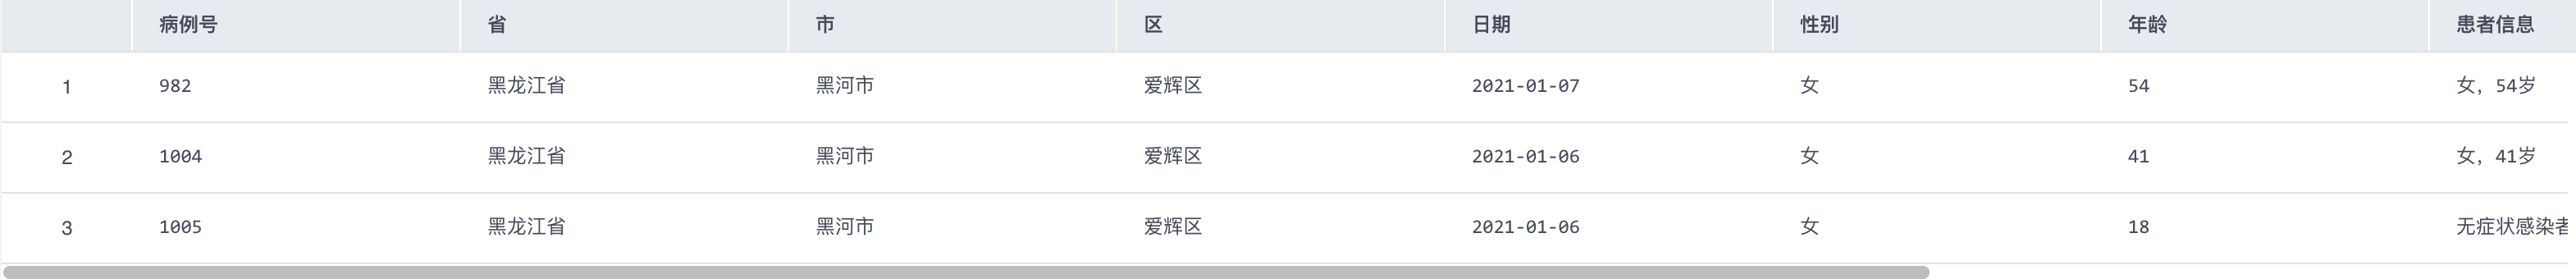
\includegraphics[width=\textwidth]{./images/lab1_query5.png}
    \caption{查询结果5\label{fig:query5}}
\end{figure}

\paragraph{石家庄市在2021年1月11日当天以及之前的所有60岁以上的患者信息} SQL语句如下:

\begin{code}
\begin{minted}{sql}
SELECT *
FROM 病例基本信息表
WHERE 日期 <= '2021-01-11' AND 市 = '石家庄市' AND 年龄 >= 60;
\end{minted}
\end{code}

语句按照给定条件筛选元组。查询到90条结果(如果条件设为\mintinline{text}{年龄 > 60}则查询到84条结果)查询结果如\figref{fig:query6}。

\begin{figure}[!htb]
    \centering
    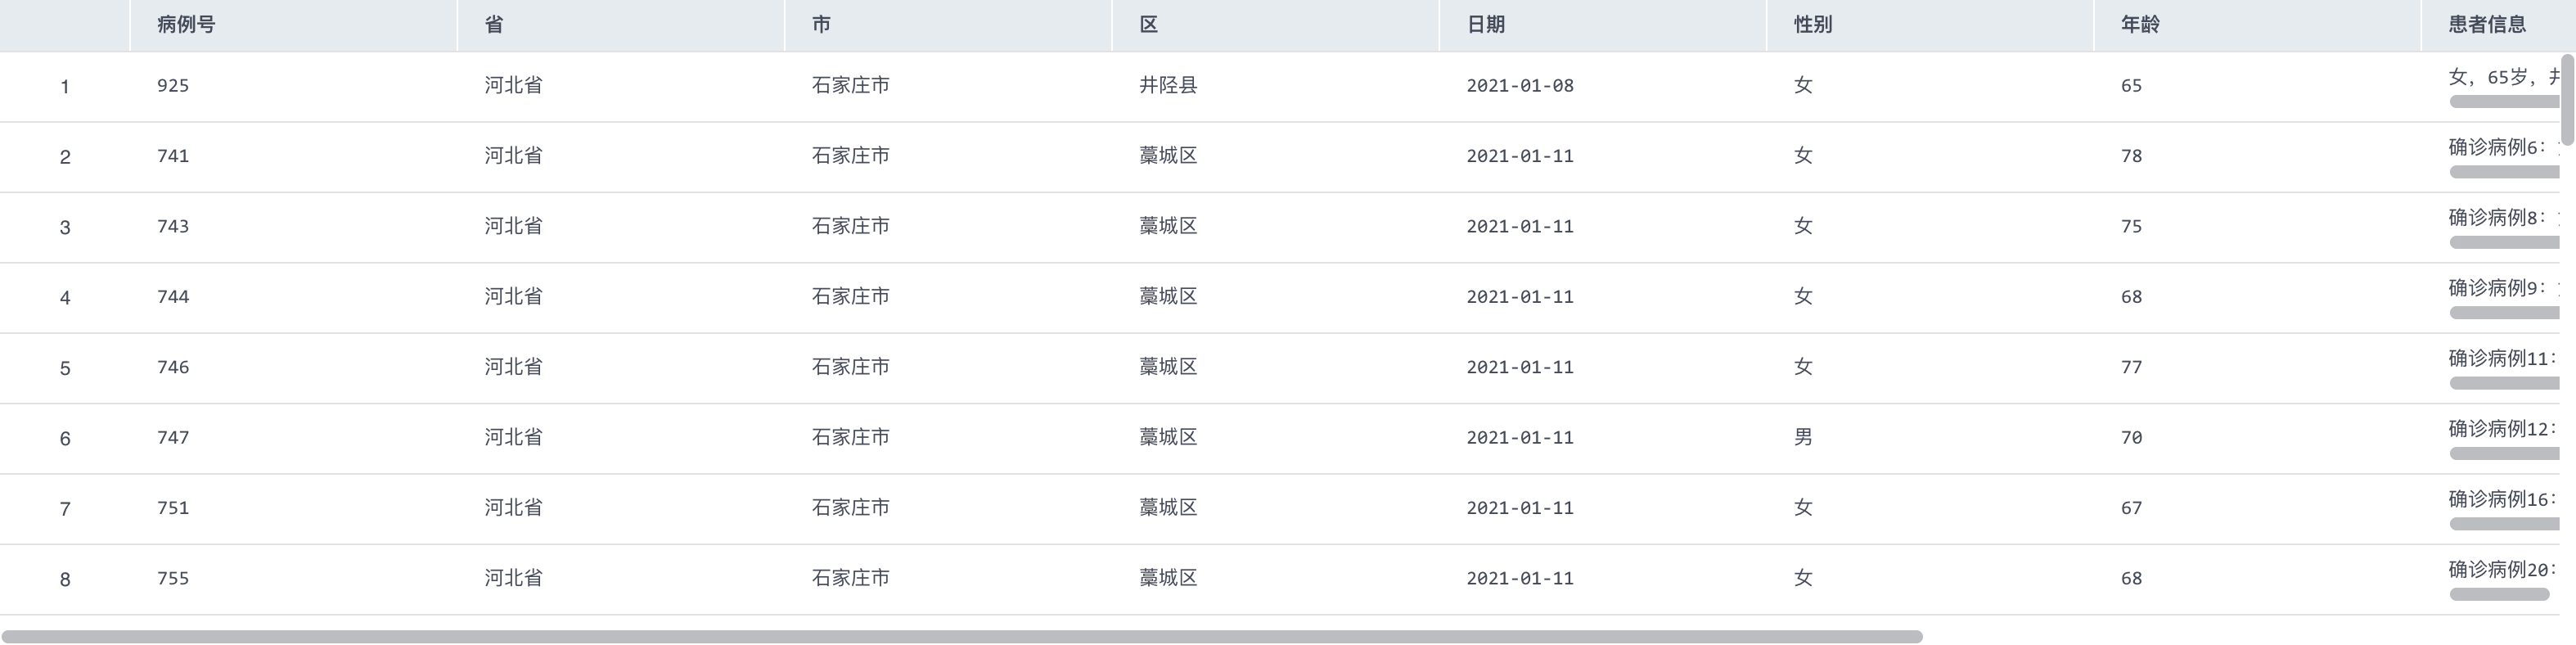
\includegraphics[width=\textwidth]{./images/lab1_query6.png}
    \caption{查询结果6\label{fig:query6}}
\end{figure}

\paragraph{截止到2020年12月30日美国累计确诊病例数最多的10个州} SQL语句如下:

\begin{code}
\begin{minted}{sql}
SELECT 州, SUM(累计确诊) AS 州累计确诊
FROM 美国各州县确诊与死亡数统计表
WHERE 日期 = '2020-12-30'
GROUP BY 州
ORDER BY 州累计确诊 DESC
LIMIT 10;
\end{minted}
\end{code}

语句筛选出当日的数据,并且按照州分组,通过累计确诊降序排列,再筛选出前十个。查询结果如\figref{fig:query7}。

\begin{figure}[!htb]
    \centering
    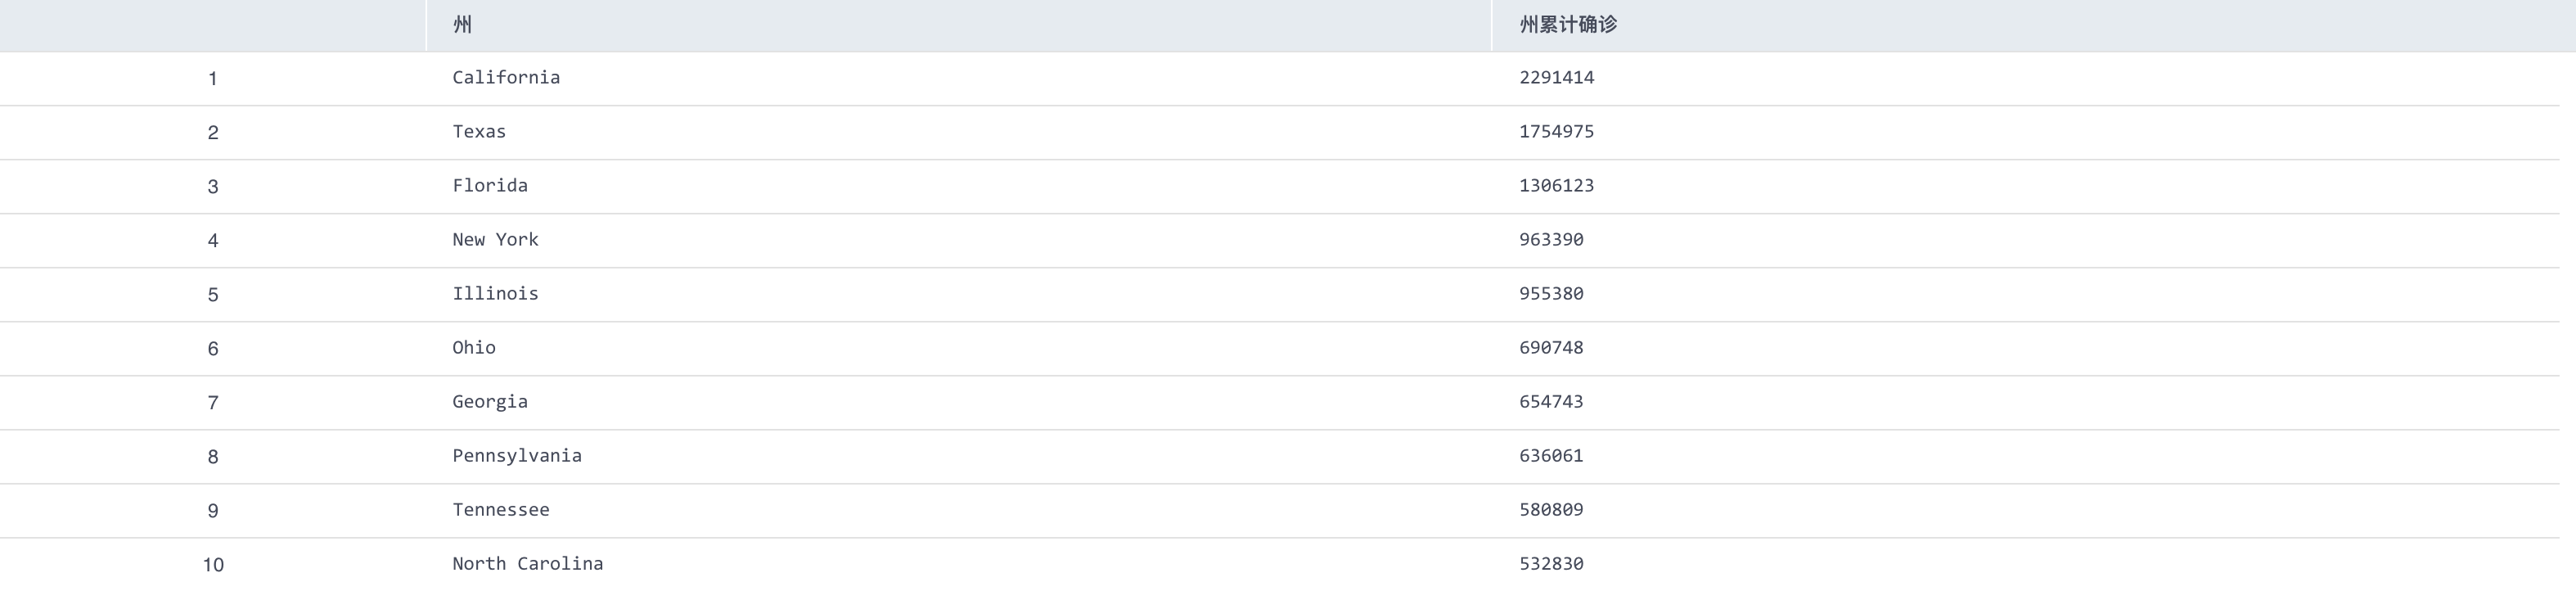
\includegraphics[width=\textwidth]{./images/lab1_query7.png}
    \caption{查询结果7\label{fig:query7}}
\end{figure}

\paragraph{截止到2020年12月30日美国新冠疫情死亡率高于2\%的州} SQL语句如下:

\begin{code}
\begin{minted}{sql}
SELECT 州, 州累计死亡/州累计确诊 AS 死亡率
FROM (
    SELECT 州, SUM(累计死亡) AS 州累计死亡, SUM(累计确诊) AS 州累计确诊
    FROM 美国各州县确诊与死亡数统计表
    WHERE 日期 = '2020-12-30'
    GROUP BY 州
)
WHERE 州累计确诊 <> 0 AND 死亡率 > 0.02;
\end{minted}
\end{code}

语句首先在FROM子查询中筛选出当日的数据,按照各州的累计死亡和累计确诊聚合,最后在外层筛选出死亡率符合条件的州。查询结果如\figref{fig:query8}。

\begin{figure}[!htb]
    \centering
    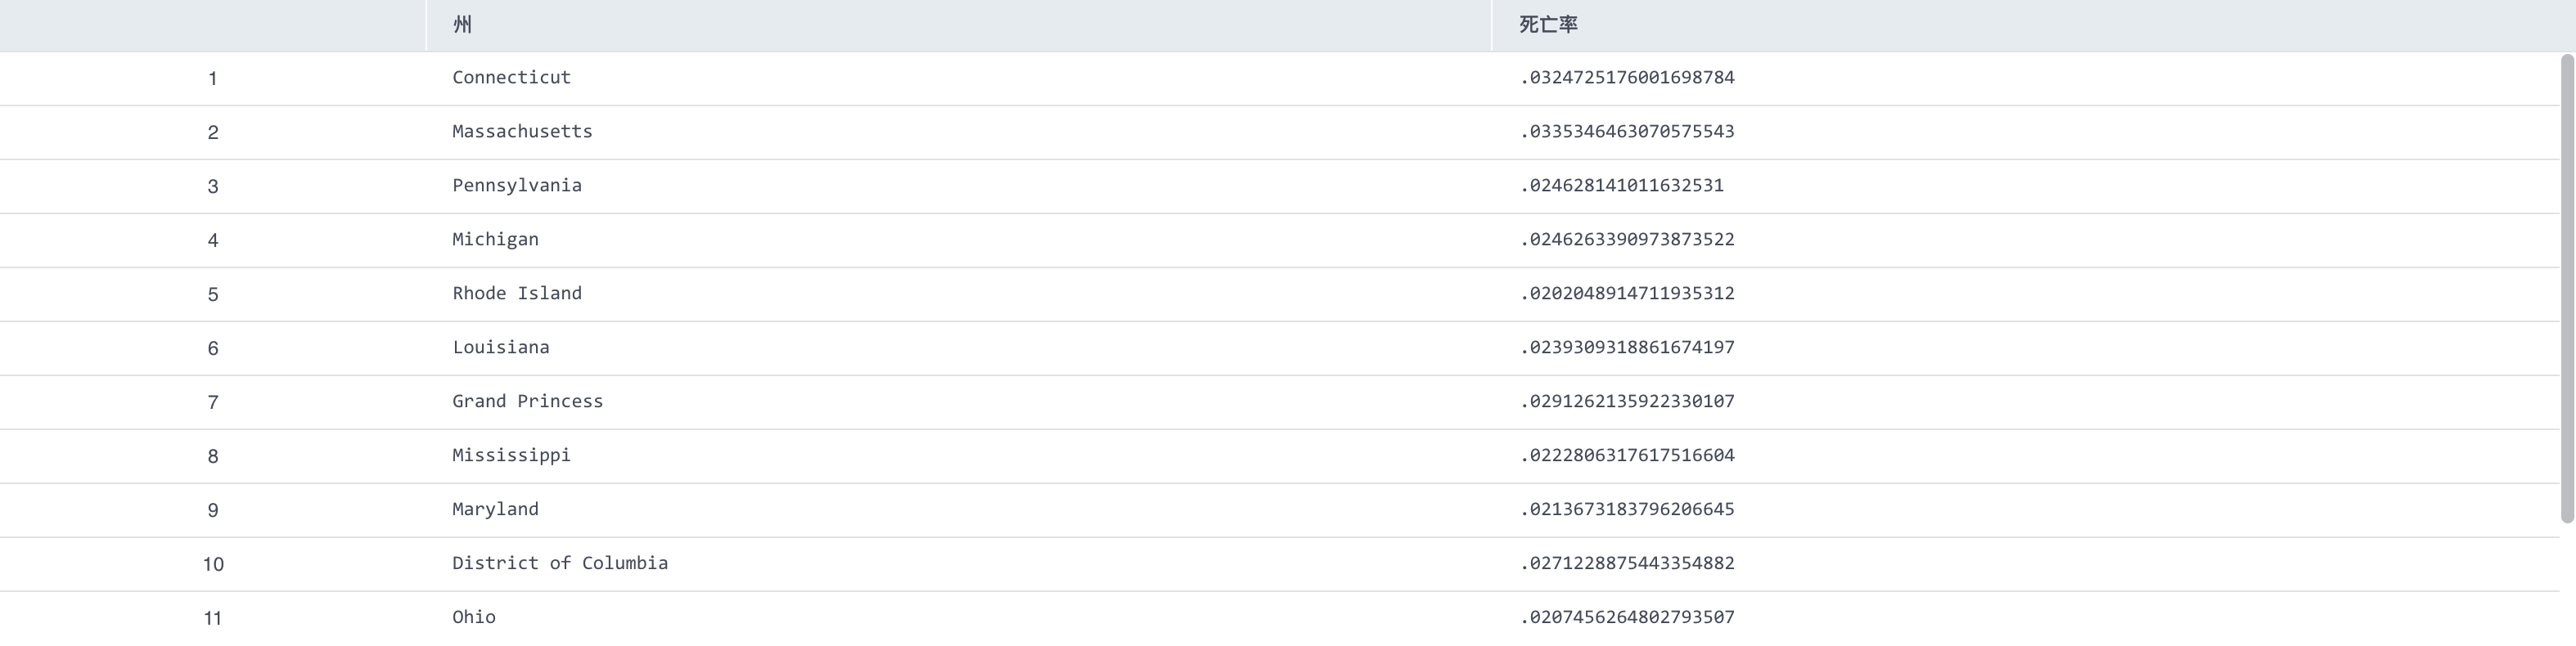
\includegraphics[width=\textwidth]{./images/lab1_query8.png}
    \caption{查询结果8\label{fig:query8}}
\end{figure}

\paragraph{曾去过“源升品质生活坊”的所有患者的基本信息} SQL语句如下:

\begin{code}
\begin{minted}{sql}
SELECT 病例基本信息表.*
FROM 病例基本信息表 NATURAL JOIN 病例行程信息表
WHERE 行程信息 LIKE '%源升品质生活坊%';
\end{minted}
\end{code}

语句从病例基本信息表和病例形成信息表的自然连接(按照病例ID连接),筛选出行程信息中含有子串“源升品质生活坊”的元组。查询结果如\figref{fig:query9}。

\begin{figure}[!htb]
    \centering
    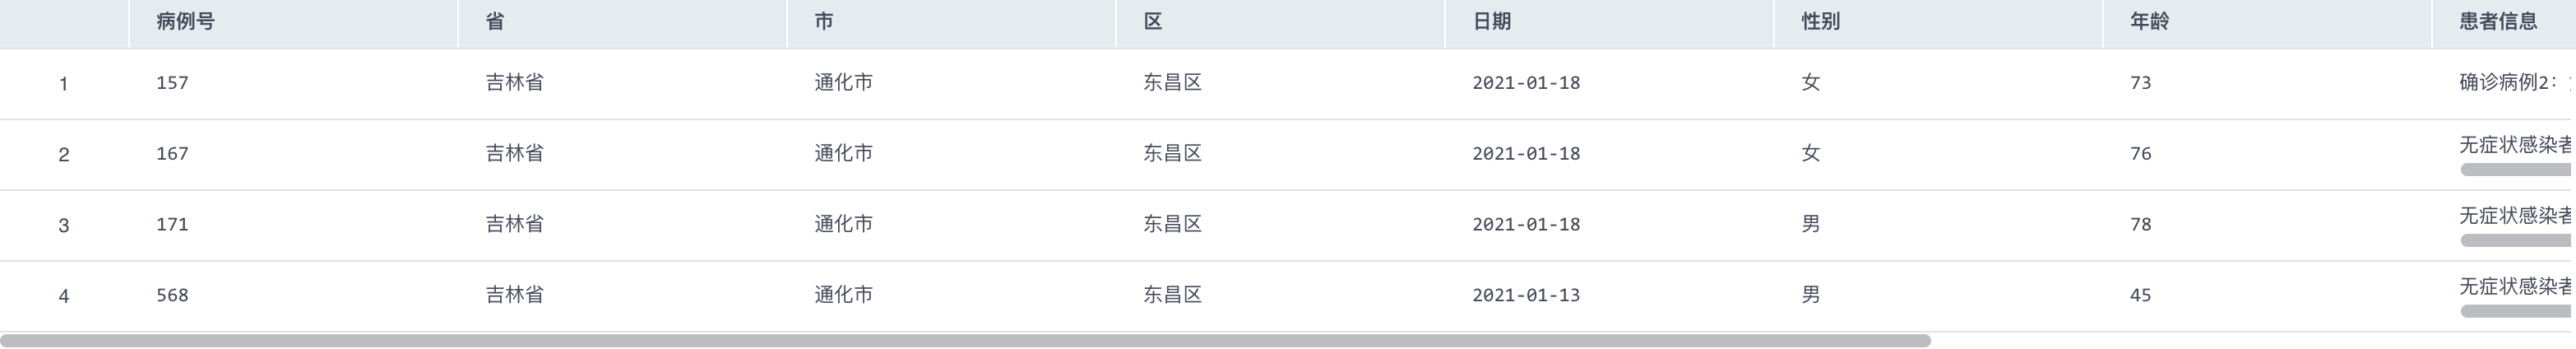
\includegraphics[width=\textwidth]{./images/lab1_query9.png}
    \caption{查询结果9\label{fig:query9}}
\end{figure}

\paragraph{行程信息中存在“家庭聚餐”的病例被确诊的日期} SQL语句如下:

\begin{code}
\begin{minted}{sql}
SELECT 日期
FROM 病例基本信息表 NATURAL JOIN 病例行程信息表
WHERE 行程信息 LIKE '%家庭聚餐%';
\end{minted}
\end{code}

与上个查询类似。查询结果如\figref{fig:query10}。

\begin{figure}[!htb]
    \centering
    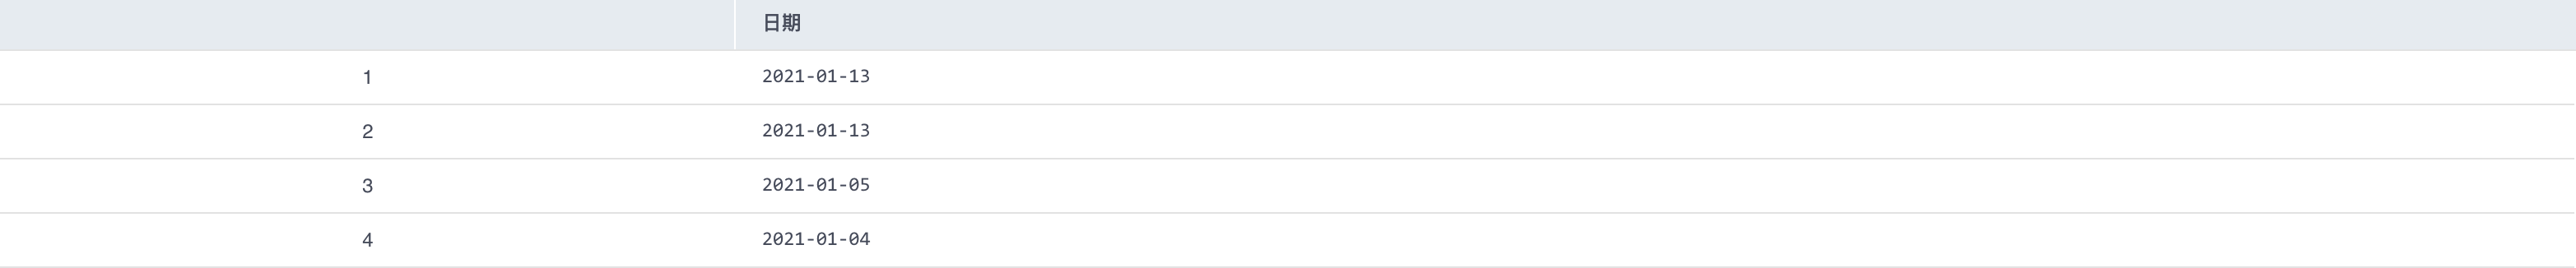
\includegraphics[width=\textwidth]{./images/lab1_query10.png}
    \caption{查询结果10\label{fig:query10}}
\end{figure}

\paragraph{对比中美两国累计确诊病例数} SQL语句如下:

\begin{code}
\begin{minted}{sql}
SELECT 日期, 中国累计确诊, 美国累计确诊
FROM (
    SELECT 日期, SUM(累计确诊) AS 中国累计确诊
    FROM 全国各省累计数据统计表
    GROUP BY 日期
) AS 中国确诊
NATURAL JOIN
(
    SELECT 日期, SUM(累计确诊) AS 美国累计确诊
    FROM 美国各州县确诊与死亡数统计表
    GROUP BY 日期
) AS 美国确诊
\end{minted}
\end{code}

语句查询中国的累计确诊信息和美国的累计确诊信息,将两个表按日期自然连接。查询结果如\figref{fig:query11}。

\begin{figure}[!htb]
    \centering
    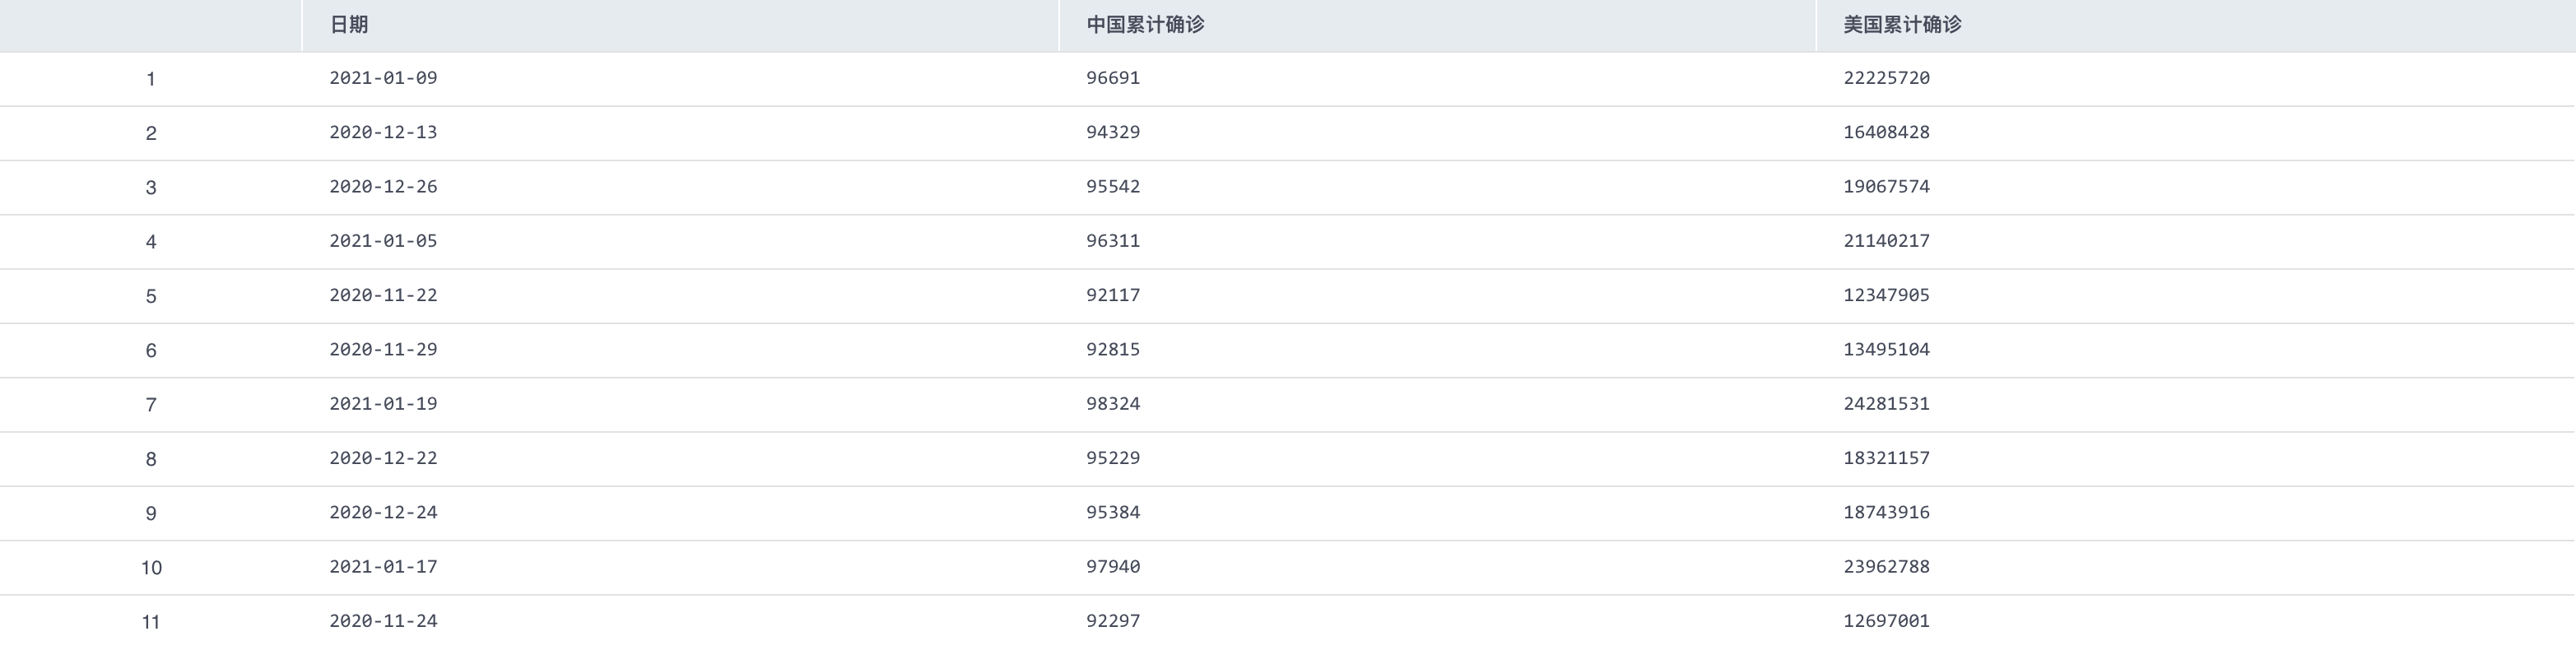
\includegraphics[width=\textwidth]{./images/lab1_query11.png}
    \caption{查询结果11\label{fig:query11}}
\end{figure}

\paragraph{截止到2021年1月20日,美国有些县的累计确诊是同一个州的其他县的2倍或以上} SQL语句如下:

\begin{code}
\begin{minted}{sql}
WITH 单日数据 AS (
    SELECT 州, 县, 累计确诊
    FROM 美国各州县确诊与死亡数统计表
    WHERE 日期 = '2021-01-20'
)
SELECT 县, 州, 州累计确诊
FROM (
    SELECT 州, SUM(累计确诊) AS 州累计确诊
    FROM 单日数据
    GROUP BY 州
) AS 州确诊
NATURAL JOIN
(
    SELECT 州, 县
    FROM 单日数据 AS T1
    WHERE 累计确诊 >= SOME (
        SELECT 累计确诊 * 2
        FROM 单日数据 AS T2
        WHERE T1.州 = T2.州
    )
) AS 确诊多的县;
\end{minted}
\end{code}

语句首先筛选出当日的各州县的累计确诊数据作为临时关系,之后利用相关子查询,筛选出确诊数比同一个州的某些县多两倍的县,将这些县与各州的总确诊数自然连接。查询结果如\figref{fig:query12}。

\begin{figure}[!htb]
    \centering
    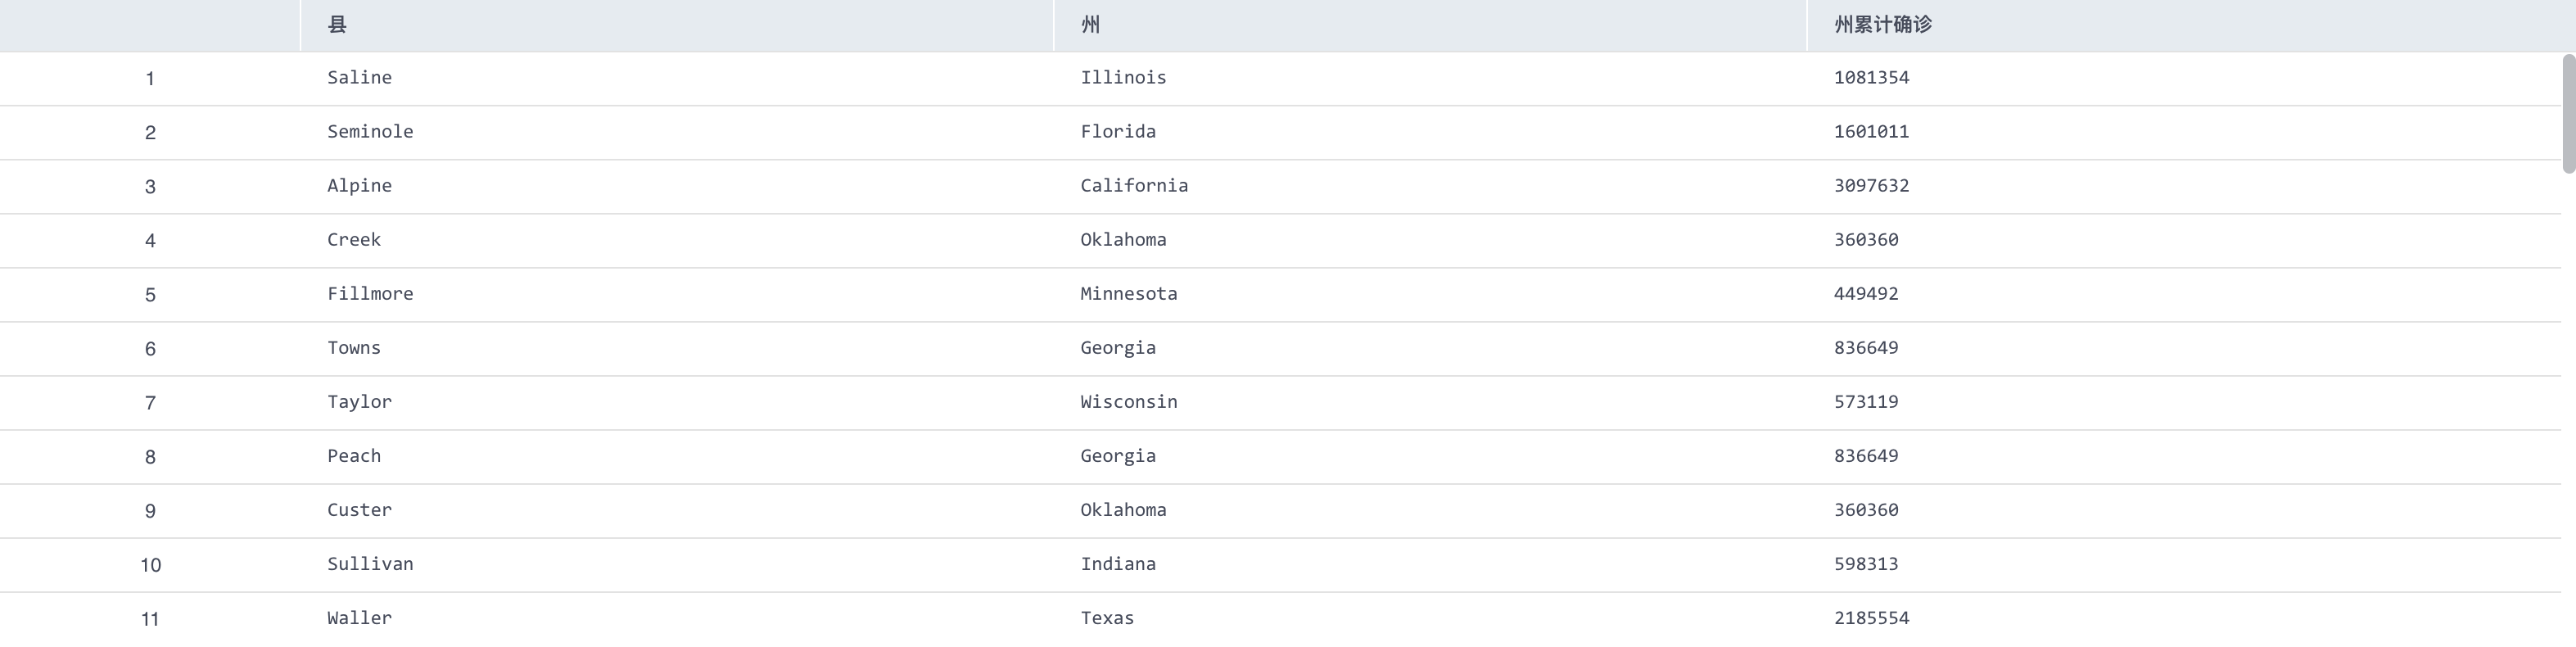
\includegraphics[width=\textwidth]{./images/lab1_query12.png}
    \caption{查询结果12\label{fig:query12}}
\end{figure}

\paragraph{世界上人口数排名前10位的国家地区} SQL语句如下:

\begin{code}
\begin{minted}{sql}
SELECT *
FROM (
    SELECT 国家地区, 人口数
    FROM 参考信息表
    WHERE 人口数 IS NOT NULL AND 组合码 = 国家地区
)
UNION 
(
    SELECT 组合码 AS 国家地区, 人口数
    FROM 全国各省参考信息表
    WHERE 组合码 = 'China'
)
ORDER BY 人口数 DESC 
LIMIT 10;
\end{minted}
\end{code}

语句提取出参考信息表中的各个国家的总人口信息,再并上中国的总人口数。查询结果如\figref{fig:query13}。

\begin{figure}[!htb]
    \centering
    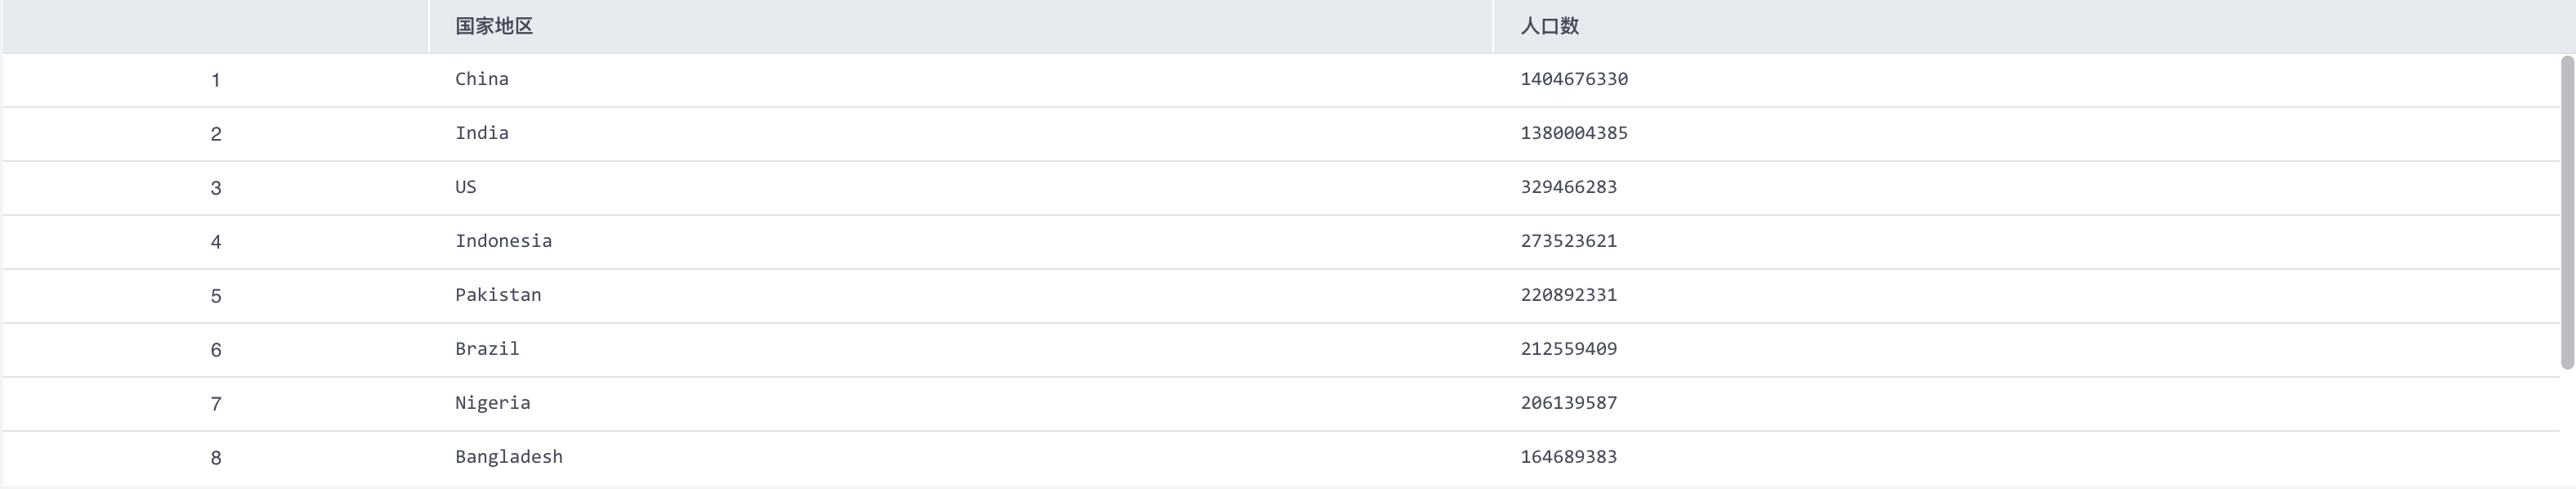
\includegraphics[width=\textwidth]{./images/lab1_query13.png}
    \caption{查询结果13\label{fig:query13}}
\end{figure}

\paragraph{美国人口超千万的大州中,截至2021年1月20日新冠肺炎疫情死亡率超过2\%的州} SQL语句如下:

\begin{code}
\begin{minted}{sql}
SELECT 州, 州累计死亡/州累计确诊 AS 死亡率
FROM (
    SELECT 州, SUM(累计死亡) AS 州累计死亡, SUM(累计确诊) AS 州累计确诊
    FROM 美国各州县确诊与死亡数统计表 AS T1
    WHERE 日期 = '2021-01-20'
    GROUP BY 州
    HAVING 10000000 < (
        SELECT 人口数
        FROM 参考信息表 AS T2
        WHERE T1.州 = T2.省州 AND T2.国家地区 = 'US' AND T2.市县 IS NULL
    )
)
WHERE 州累计确诊 <> 0 AND 死亡率 > 0.02;
\end{minted}
\end{code}

语句基于之前的查询,再在\mintinline{sql}{FROM}子查询中添加人口数超过千万的限制,这一限制通过相关子查询实现。查询结果如\figref{fig:query14}。

\begin{figure}[!htb]
    \centering
    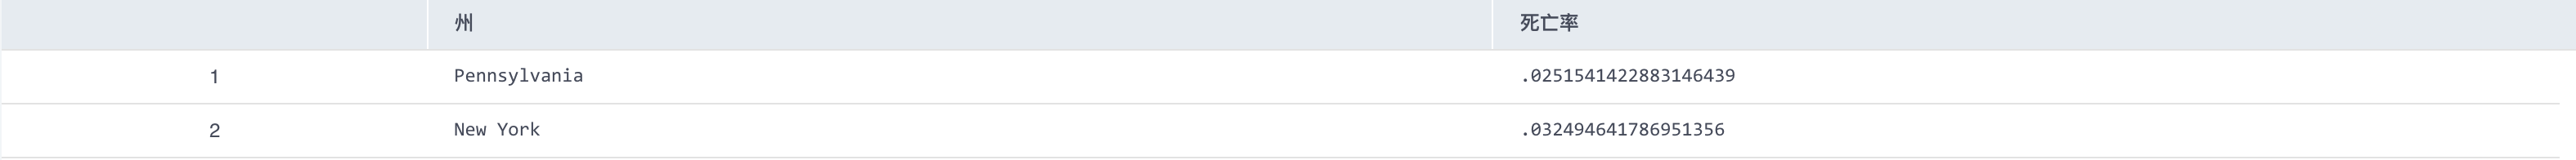
\includegraphics[width=\textwidth]{./images/lab1_query14.png}
    \caption{查询结果14\label{fig:query14}}
\end{figure}

\paragraph{截至2021年1月20日,河北省出现了新冠确诊病例但不属于中高风险的地区} SQL语句如下:

\begin{code}
\begin{minted}{sql}
SELECT DISTINCT 区
FROM 病例基本信息表
WHERE 日期 < '2021-01-20' AND 省 = '河北省' AND 区 IS NOT NULL
EXCEPT 
SELECT DISTINCT 区
FROM 全国城市风险等级表
WHERE 省 = '河北省'
\end{minted}
\end{code}

或

\begin{code}
\begin{minted}{sql}
SELECT DISTINCT 区
FROM 病例基本信息表
WHERE 日期 < '2021-01-20' AND 省 = '河北省' AND 区 IS NOT NULL AND 区 NOT IN (
    SELECT DISTINCT 区
    FROM 全国城市风险等级表
    WHERE 省 = '河北省'
);
\end{minted}
\end{code}

语句用出现确诊病例的区的集合减去中高风险地区集合,可以直接用\mintinline{sql}{EXCEPT}实现,也可以用\mintinline{sql}{NOT IN}实现。查询结果如\figref{fig:query15}。

\begin{figure}[!htb]
    \centering
    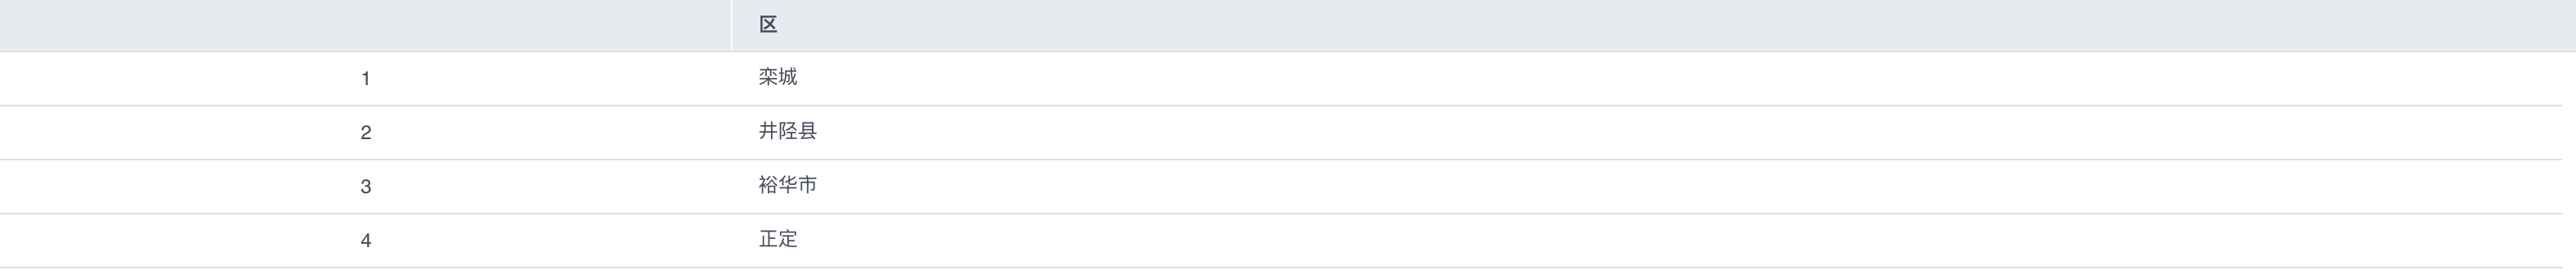
\includegraphics[width=\textwidth]{./images/lab1_query15.png}
    \caption{查询结果15\label{fig:query15}}
\end{figure}

\paragraph{在病例行程信息表的基础上根据病例基本信息表,查询河北省病例的信息} SQL语句如下:

\begin{code}
\begin{minted}{sql}
SELECT 行程号, 病例号, 患者信息, 日期信息, 行程信息
FROM 病例基本信息表 NATURAL JOIN 病例行程信息表 
WHERE 省 = '河北省';
\end{minted}
\end{code}

语句将两个表自然连接,筛选出河北省病例的信息。查询结果如\figref{fig:query16}。

\begin{figure}[!htb]
    \centering
    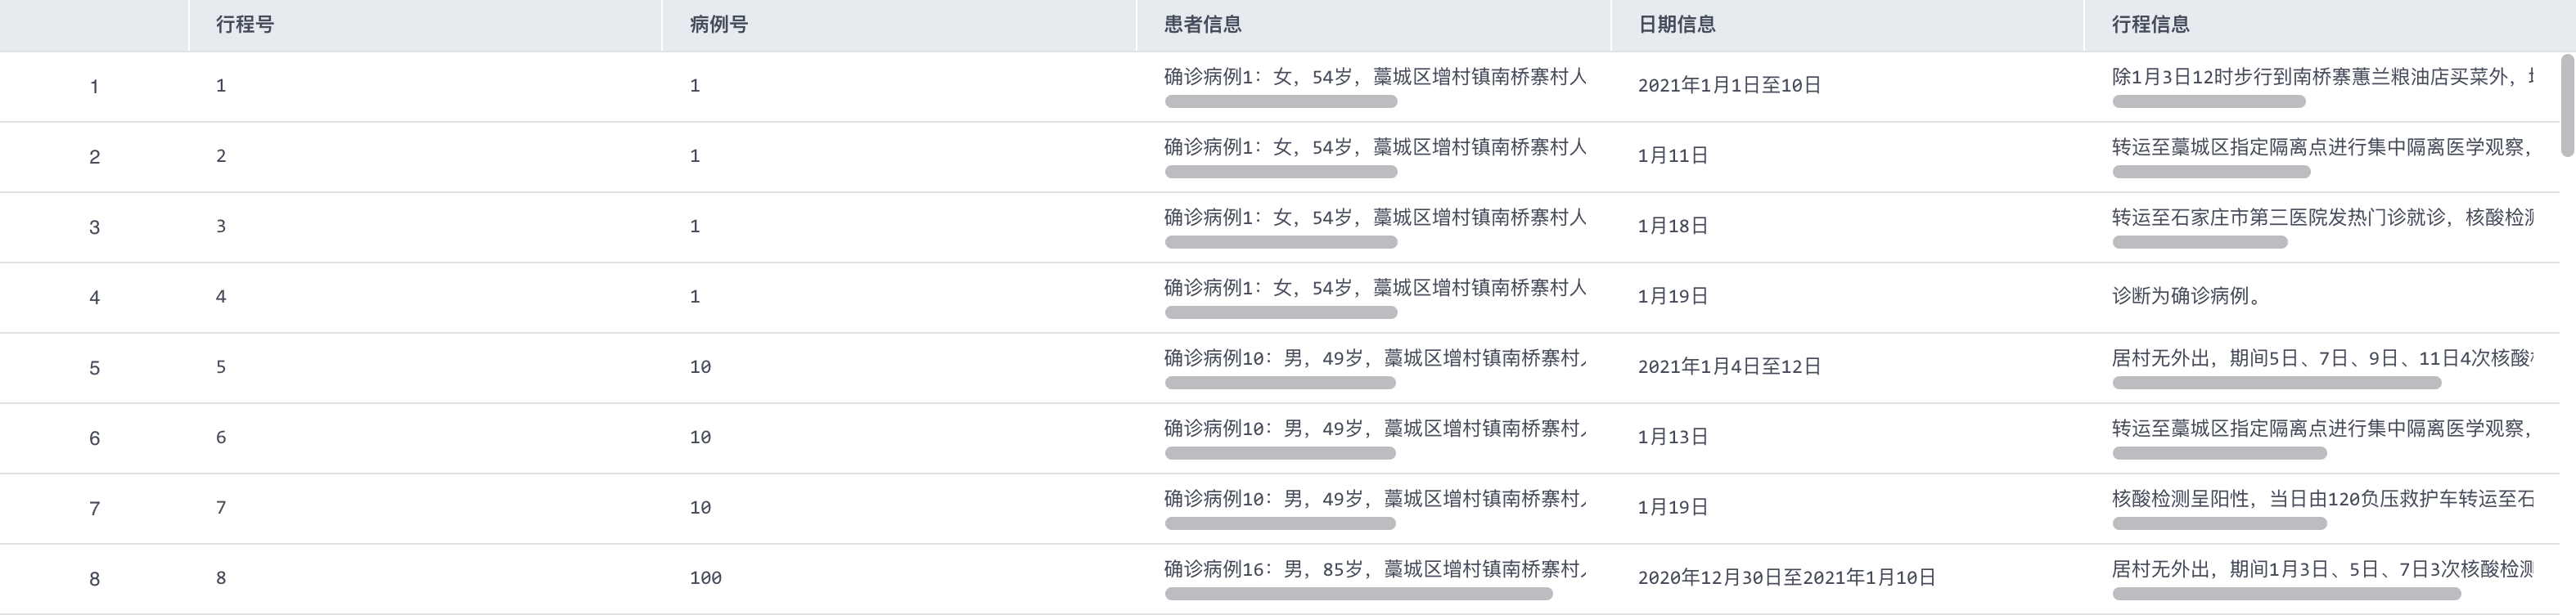
\includegraphics[width=\textwidth]{./images/lab1_query16.png}
    \caption{查询结果16\label{fig:query16}}
\end{figure}

\paragraph{查询披露的确诊患者信息中年龄最大的患者} SQL语句如下:

\begin{code}
\begin{minted}{sql}
SELECT 性别, 年龄, 患者信息
FROM 病例基本信息表
WHERE 年龄 >= ALL (
    SELECT 年龄
    FROM 病例基本信息表
    WHERE 年龄 IS NOT NULL 
)
\end{minted}
\end{code}

语句将确诊病例的信息与其他所有病例的年龄比较,找到大于等于所有其他患者年龄的患者。查询结果如\figref{fig:query17}。

\begin{figure}[!htb]
    \centering
    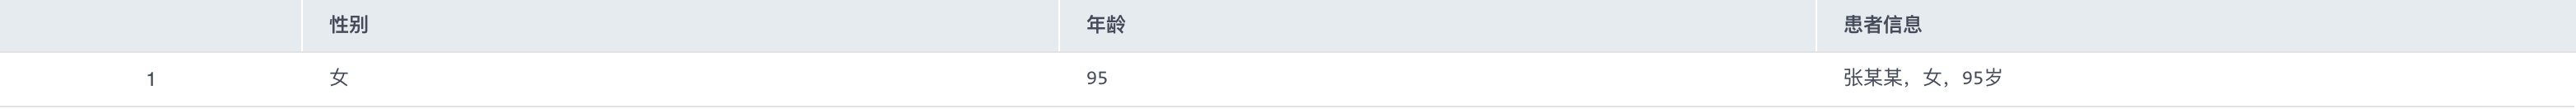
\includegraphics[width=\textwidth]{./images/lab1_query17.png}
    \caption{查询结果17\label{fig:query17}}
\end{figure}

\paragraph{2020年12月份新增确诊患者最多的城市} SQL语句如下:

\begin{code}
\begin{minted}{sql}
WITH 十二月各市确诊 AS (
    SELECT 市, COUNT(*) AS 病例数
    FROM 病例基本信息表
    WHERE 日期 BETWEEN '2020-12-01' AND '2020-12-31'
    GROUP BY 市
)
SELECT *
FROM 十二月各市确诊
WHERE 病例数 >= ALL (
    SELECT 病例数
    FROM 十二月各市确诊
)
\end{minted}
\end{code}

语句首先建立十二月各个市确诊的临时关系,之后选出病例数大于其他所有城市的城市。查询结果如\figref{fig:query18}。

\begin{figure}[!htb]
    \centering
    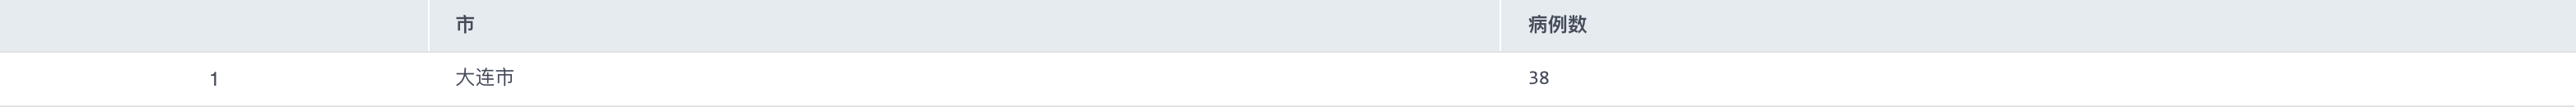
\includegraphics[width=\textwidth]{./images/lab1_query18.png}
    \caption{查询结果18\label{fig:query18}}
\end{figure}

\paragraph{没有新增确诊病例或未披露病例信息的省份} SQL语句如下:

\begin{code}
\begin{minted}{sql}
SELECT 中文名称 AS 省
FROM 全国各省参考信息表
WHERE 中文名称 IS NOT NULL 
EXCEPT
SELECT DISTINCT 省
FROM 病例基本信息表
\end{minted}
\end{code}

用集合的差实现。查询到21条结果,查询结果如\figref{fig:query19}。

\begin{figure}[!htb]
    \centering
    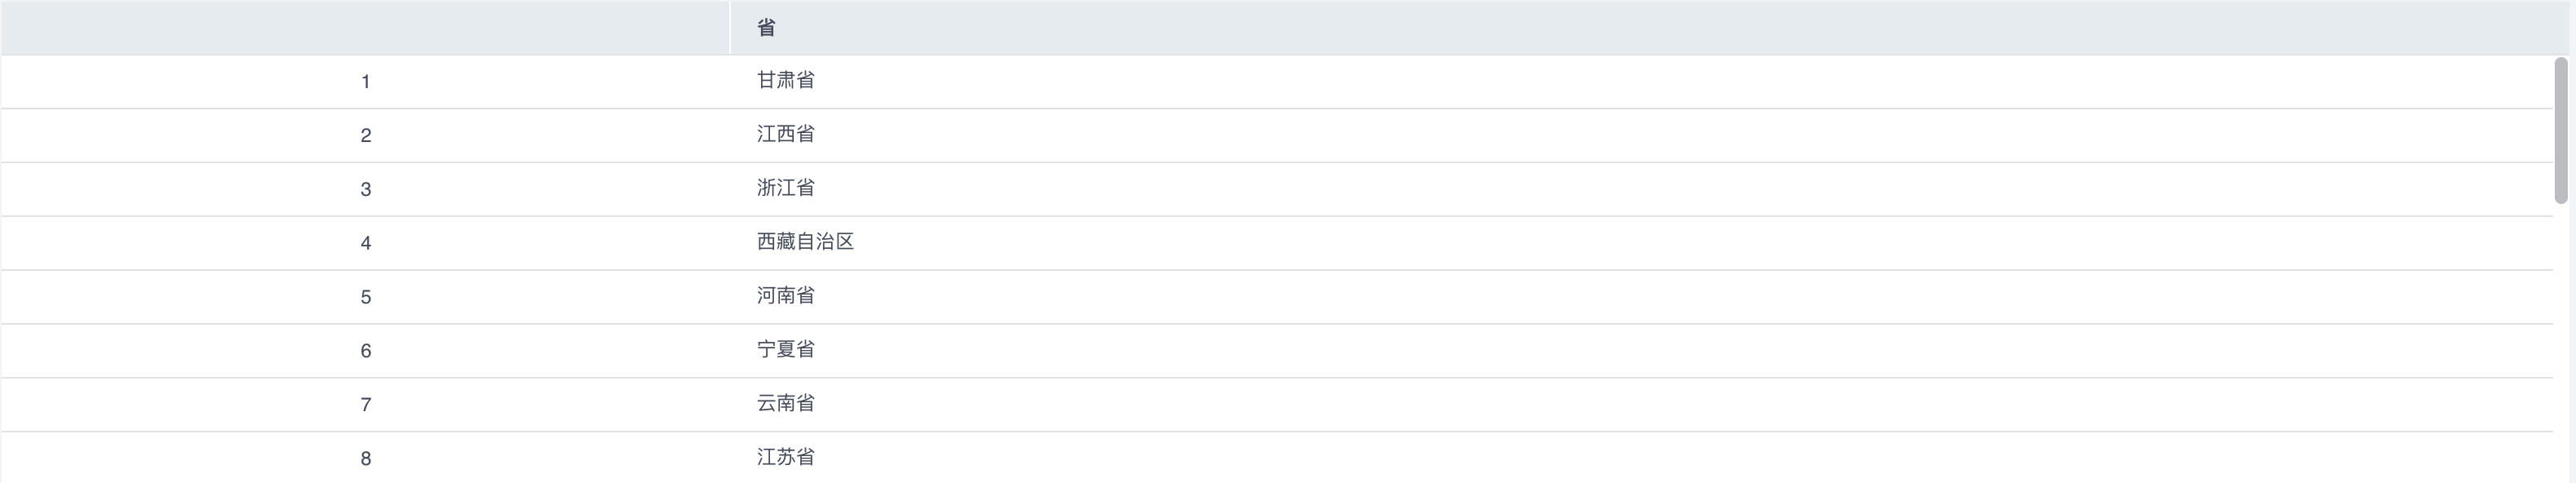
\includegraphics[width=\textwidth]{./images/lab1_query19.png}
    \caption{查询结果19\label{fig:query19}}
\end{figure}

\paragraph{全国中高风险地区所在省中,在2021年1月20日没有新增确诊信息披露的} SQL语句如下:

\begin{code}
\begin{minted}{sql}
SELECT DISTINCT 省
FROM 全国城市风险等级表
EXCEPT 
SELECT DISTINCT 省
FROM 病例基本信息表
WHERE 日期 = '2021-01-20'
\end{minted}
\end{code}

用集合的差实现。查询结果如\figref{fig:query20}。

\begin{figure}[!htb]
    \centering
    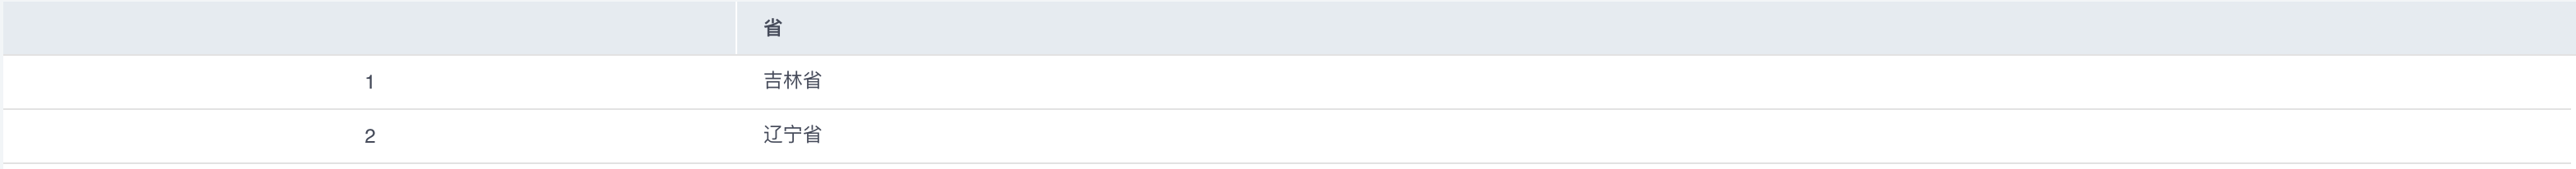
\includegraphics[width=\textwidth]{./images/lab1_query20.png}
    \caption{查询结果20\label{fig:query20}}
\end{figure}

\paragraph{一月份国内新增患者病例最多的城市} SQL语句如下:

\begin{code}
\begin{minted}{sql}
WITH 一月各市确诊 AS (
    SELECT 市, COUNT(*) AS 病例数
    FROM 病例基本信息表
    WHERE 日期 BETWEEN '2021-01-01' AND '2021-01-31'
    GROUP BY 市
)
SELECT *
FROM 一月各市确诊
WHERE 病例数 >= ALL (
    SELECT 病例数
    FROM 一月各市确诊
)
\end{minted}
\end{code}

和查询18一致。查询结果如\figref{fig:query21}。

\begin{figure}[!htb]
    \centering
    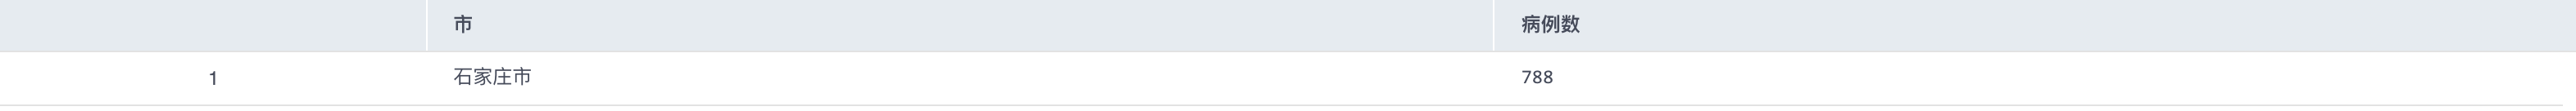
\includegraphics[width=\textwidth]{./images/lab1_query21.png}
    \caption{查询结果21\label{fig:query21}}
\end{figure}

\paragraph{除中美两国以外的其余国家中,进入2021年以来单日新增确诊病例始终不低于一万例的国家} SQL语句如下:

\begin{code}
\begin{minted}{sql}
WITH 排除中美的国家 AS (
    SELECT 日期, 国家地区, SUM(累计确诊) AS 国家累计确诊
    FROM 各国疫情数据统计表 S
    WHERE 日期 >= '2020-12-31' AND 国家地区 NOT IN ('US', 'China') AND NOT EXISTS (
        SELECT *
        FROM 各国疫情数据统计表 T
        WHERE S.国家地区 = T.国家地区 AND T.省州 IS NULL
    )
    GROUP BY 日期, 国家地区
    UNION
    SELECT 日期, 国家地区, 累计确诊 AS 国家累计确诊
    FROM 各国疫情数据统计表
    WHERE 日期 >= '2020-12-31' AND 国家地区 NOT IN ('US', 'China') AND 省州 IS NULL
)
SELECT DISTINCT 国家地区
FROM 排除中美的国家 AS S
WHERE 10000 <= ALL (
    SELECT T2.国家累计确诊 - T1.国家累计确诊
    FROM 排除中美的国家 AS T1 JOIN 排除中美的国家 AS T2 USING (国家地区)
    WHERE T2.日期 = T1.日期 + 1 AND T1.国家地区 = S.国家地区
)
\end{minted}
\end{code}

语句首先筛选出除了中美的国家在一月的累计确诊信息,由于有的国家的总确诊数已经给出,而另一些需要通过求各个地区确诊数的和来求出,因此需要求两个集合的并。最后从这些数据中通过两个关系算出某个国家每相邻两天确诊数的差值,并且要求这些差值都大于10000。查询结果如\figref{fig:query22}。

\begin{figure}[!htb]
    \centering
    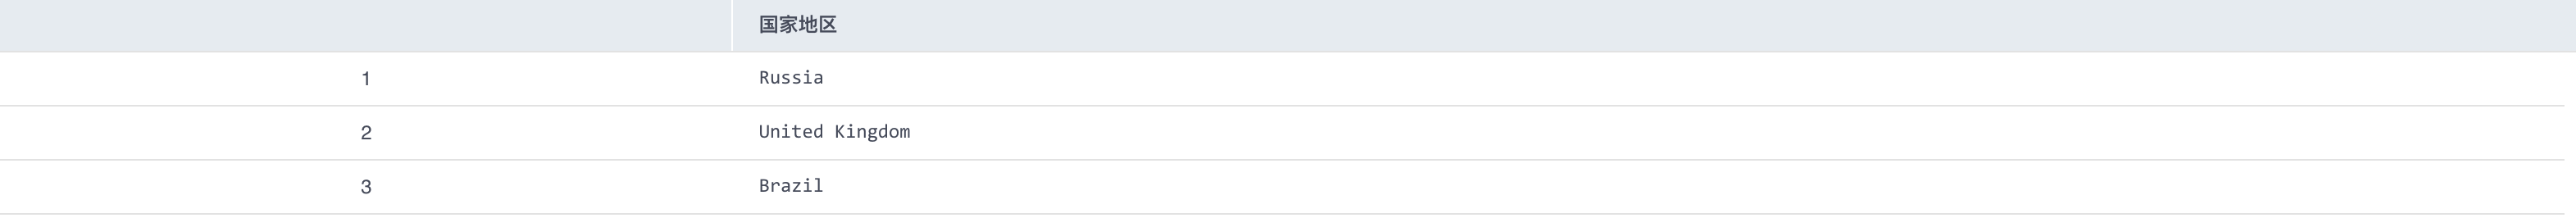
\includegraphics[width=\textwidth]{./images/lab1_query22.png}
    \caption{查询结果22\label{fig:query22}}
\end{figure}

\section{实验总结}

在实验的过程中,主要涉及的SQL语法错误如下:

\begin{itemize}
    \item 用单引号括起字符串;
    \item 子查询的列名和外部查询的列名重复;
    \item \mintinline{sql}{WHERE}子句中试图访问\mintinline{sql}{FROM}子句中未指明的关系;
    \item \mintinline{sql}{WHERE}子句中试图声明别名;
    \item 子查询连接时未声明别名。
\end{itemize}

另外,需要观察数据足够细致才能注意到有些数据中不需要聚合求和而另一些数据中需要。

实验中,我参考PostgreSQL的语法说明和教材上的内容编写SQL语句,使我对SQL语法的熟悉程度大大增加,同时增强了我的英文文献阅读能力,我收获颇丰。

\end{document}